%%%%%%%%%%%%%%%%%%%%%%%%%%%%%%%%%%%%%%%%%%%%%%%%%%%%%%
%% "Magic comments" for the LaTeX editor -------------
% !TEX root = ../Diss.tex
%%%%%%%%%%%%%%%%%%%%%%%%%%%%%%%%%%%%%%%%%%%%%%%%%%%%%%
%
\begin{showExamples}%
%
%%%%%%%%%%%%%%%%%%%%%%%%%%%%%%%%%%%%%%%%%%%%%%%%%%%%%%%%%%%%
\chapter{Anleitung zur Nutzung dieser Vorlage}%
\label{chap:Examples}
%%%%%%%%%%%%%%%%%%%%%%%%%%%%%%%%%%%%%%%%%%%%%%%%%%%%%%%%%%%%
%
%
Dieses Kapitel zeigt den grundlegenden Aufbau eines einfachen Kapitels.
Die einzelnen Abschnitte beschreiben die Struktur der Vorlage und geben wichtige allgemeine Tipps.
Die Verwendung einzelner Features dieser Vorlage wird in \cref{chap:Examples} detailliert beschrieben und demonstriert.

Es wird empfohlen, die einzelnen Unterkapiteln jedes Kapitels als eigene Dateien anzulegen und sie mit dem \verb+\input{}+-Befehl einzubinden (s. Quelltext).
Dies erlaubt die einzelnen Unterkapitel bei Bedarf leichter zu verschieben oder mit einem einzigen \%-Zeichen temporär auszukommentieren und erleichtert so die Fehlersuche.

Zur Nutzung dieser Vorlage für die eigene Arbeit empfiehlt es sich, die Anleitungskapiteln auszublenden und ansonsten die bestehende Struktur zu nutzen.
Die Anleitungskapiteln lassen sich ausblenden, indem man in der Datei
\printfilepath{preambel/AlleSchalter.tex} in der Zeile
\lstinline|\setUserDefinedBoolean{showExamples}{true}| 
den Wert \printkeyword{true} durch \printkeyword{false} ersetzt.
Ähnlich lassen sich auch andere Teile des Manuskriptes ausblenden ohne sie auskommentieren zu müssen.%
%
\footnote{Die Befehle
\lstinline|\setUserDefinedBoolean{IrgendeinName}{Bool-Wert}| 
sind spezielle Makros, die jeweils eine Boolean-Variable mit dem entsprechenden Wert definieren,
sowie eine \LaTeX"=Umgebung \printkeyword{IrgendeinName},
deren Inhalt von LaTeX{} angezeigt bzw. ausgeblendet wird.
Dies betrifft alles, was im weiteren \LaTeX-Quellcode zwischen
\lstinline|\begin{IrgendeinName}| und \lstinline|\end{IrgendeinName}| steht.
Der Vorteil dieser Vorgehensweise gegenüber einem einfachen Auskommentieren liegt bei Einbindung von Dateien darin,
dass die zwischen
\lstinline|\begin{IrgendeinName}| und \lstinline|\end{IrgendeinName}|
eingebundenen Dateien weiterhin im Verzeichnisbaum vom TeXnicCenter etc.
sichtbar bleiben und bei Bedarf schnell als Referenz aufgerufen werden können.}
%
%%%%%%%%%%%%%%%%%%%%%%%%%%%%%%%%%%%%%%%%%%%%%%%%%%%%%%%%%%%%
\section{Kompilierung der Vorlage}%
\label{sec:Kompilierung}
%%%%%%%%%%%%%%%%%%%%%%%%%%%%%%%%%%%%%%%%%%%%%%%%%%%%%%%%%%%%
%
Um diese Vorlage nutzen zu können, benötigt man eine \LaTeX-Distribution (z.B. \printswname{MiKTeX}\footnote{\url{http://www.miktex.org/}} oder \printswname{TeXLive}\footnote{\url{https://tug.org/texlive/acquire.html}}).
Sofern man nicht die riesengroße Komplettinstallation wählt, wird beim ersten Kompilieren eine Internet"=Verbindung benötigt, um Zusatz"=\glspl{gls:pkg} dynamisch nachladen zu können.
Zur Erstellung des Glossars und des Abkürzungsverzeichnisses wird zusätzlich Perl benötigt.
Unter Windows müsste hierzu zusätzlich beispielsweise \printswname{ActivePerl}\footnote{\url{https://www.activestate.com/products/activeperl/}}
oder \printswname{StrawberryPerl}\footnote{\url{http://strawberryperl.com/}} installiert werden.
Bei den Linux-Distributionen ist Perl automatisch mit dabei.

Zur bequemen Bearbeitung der \LaTeX"=Quellcode"=Dateien empfiehlt sich Verwendung einer guten \LaTeX"=Entwicklungsumgebung in Kombination mit einem geeigneten, sprich SyncTeX"=fähigen, PDF"=Betrachter.
Manche Entwicklungsumgebungen bieten eine integrierte PDF"=Vorschau, welche Vor- und Nachteile haben kann.
Ein wichtiges Kriterium bei der Wahl der Entwicklungsumgebung ist die Möglichkeit, zwischen den einzelnen Stellen im Quellcode und im PDF hin- und her springen zu können.
Unter Windows war lange Zeit \textbf{TeXnicCenter}\footnote{\url{http://www.texniccenter.org/}} in Kombination mit \printswname{SumatraPDF}\footnote{\url{https://www.sumatrapdfreader.org}} eine gute Wahl gewesen.
Mittlerweile tendieren die meisten dazu, \printswname{TeXstudio}\footnote{\url{https://www.texstudio.org/}} zu verwenden.
Diese bietet eine eingebaute PDF"=Vorschau und viele nützliche Features und ist sowohl unter Windows als auch unter Linux verfügbar.

%%%%%%%%%%%%%%%%%%%%%%%%%%%%%%%%%%%%%%%%%%%%%%%%%%%%%%%%%%%%
\subsection{MiKTeX-Einstellungen}
\label{sec:MiKTeX}
%%%%%%%%%%%%%%%%%%%%%%%%%%%%%%%%%%%%%%%%%%%%%%%%%%%%%%%%%%%%
Sofern MiKTeX als \LaTeX"=Distribution verwendet wird, sollte man darauf achten, dass bei Bedarf Zusatzpakete vom Internet dynamisch nachgeladen werden können.
Sofern diese Option nicht bei der Installation gesetzt worden ist, kann sie nachträglich in der MiKTeX-Console aktiviert werden.
Zu finden ist diese im Startmenü unter \enquote{MiKTeX}, \enquote{MiKTeX Console (Admin)}.
Unter \enquote{Settings} findet sich ein Reiter \enquote{General}, wo im Bereich \enquote{Package installation} entweder die Option \enquote{Always install missing packages on the fly} oder \enquote{Ask me} ausgewählt werden soll.
Sofern sich der Rechner im Netzwerk des Fraunhofer IOSB befindet, muss zusätzlich noch die Proxy-Option korrekt gesetzt werden.
Hierfür muss man im Bereich \enquote{Package installation} der MiKTeX Console auf \enquote{Change} gehen und bei \enquote{Connection Settings} die Verwendung des Proxy-Servers \printkeyword{proxy-ka.iosb.fraunhofer.de} mit Port \printkeyword{80} aktivieren (s. \cref{fig:MiKTeX-Proxy}).
Wird dies nicht gemacht, können benötigte Pakete nicht nachgeladen werden.

\begin{figure}[htb]%
\centering%
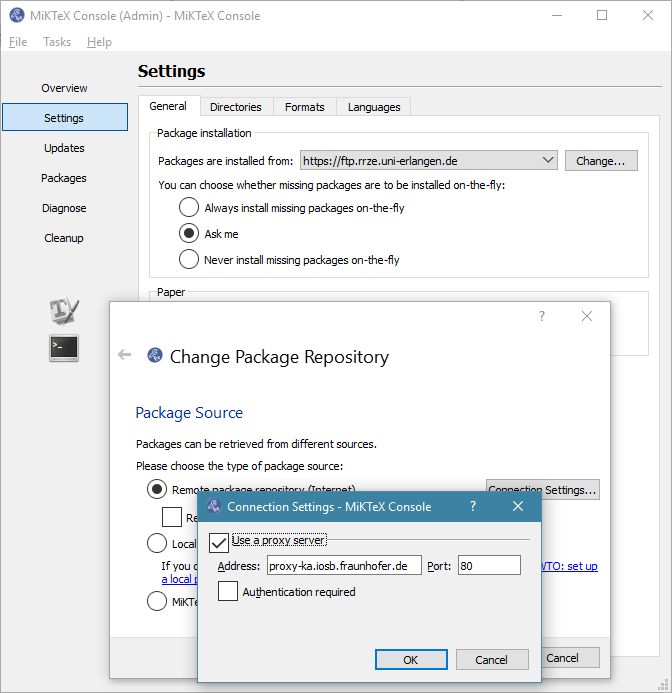
\includegraphics[width=\linewidth]{images/examples/MiKTeX-Proxy.png}%
\caption{MiKTeX-Einstellungen zum Nachladen der Zusatzpakete}%
\label{fig:MiKTeX-Proxy}%
\end{figure}

Nach der MiKTeX-Installation sollte man im Startmenü gleich die MiKTeX-Console aufrufen, den Proxy eintragen und das Update durchführen um die aktuellste Version der vorinstallierten Pakete zu erhalten.
So vermeidet man beim automatischen Nachladen weiterer \glspl{gls:pkg} aus dem \acrshort{ac:CTAN}-Repository etwaige Inkompatibilitäten aufgrund veralteter Stammpakete.


%%%%%%%%%%%%%%%%%%%%%%%%%%%%%%%%%%%%%%%%%%%%%%%%%%%%%%%%%%%%
\subsection{TeXLive-Einstellungen}
\label{sec:TeXLive}
%%%%%%%%%%%%%%%%%%%%%%%%%%%%%%%%%%%%%%%%%%%%%%%%%%%%%%%%%%%%
Bei Verwendung von TeXLive unter Linux muss darauf geachtet werden, dass alle notwendigen Linux-\glspl{gls:pkg} installiert sind.
Unter Ubuntu 17.04 sollte es funktionieren, wenn folgende Linux-\glspl{gls:pkg} installiert wurden:
\begin{itemize*}
	\item {\small\verb#texlive#}
	\item {\small\verb#texlive-lang-german#}
	\item {\small\verb#texlive-fonts-extra#}
	\item {\small\verb#texlive-bibtex-extra#}
	\item {\small\verb#fonts-linuxlibertine#}
	\item {\small\verb#biber#}
	\item {\small\verb#xindy#}
	\item {\small\verb#texmaker#}
\end{itemize*}
Texmaker ist eine IDE für \LaTeX, die aber vermutlich über Dependencies schon einige Pakete mitbringt.


%%%%%%%%%%%%%%%%%%%%%%%%%%%%%%%%%%%%%%%%%%%%%%%%%%%%%%%%%%%%
\subsection{Kompilieraufrufe}
\label{sec:Aufruf}
%%%%%%%%%%%%%%%%%%%%%%%%%%%%%%%%%%%%%%%%%%%%%%%%%%%%%%%%%%%%
Zur erfolgreichen Kompilierung des Dokumentes müssen mehrere
Kommandozeilenprogramme aufgerufen werden.
Bei Verwendung einer integrierten Entwicklungsumgebung (IDE),
wird diese so konfiguriert, dass die Aufrufe aus der IDE heraus erfolgen und
die etwaigen Warnungen, Erfolgs- und Fehlermeldungen in der IDE sichtbar werden.
Die entsprechenden Einstellungen für TeXnicCenter und TeXstudio finden sich
in den nachfolgenden Kapiteln.

Die einzelnen Aufrufe sind:
\begin{itemize*}
\item \index{xelatex}\texttt{xelatex} zur eigentlichen Kompilierung von \LaTeX-Quelltext,
\item \index{biber}\texttt{biber} zur Kompilierung von Bibliografien,
\item \index{makeglossaries}\texttt{makeglossaries}, welches intern \index{xindy}\texttt{xindy} aufruft,
zur Erstellung einer Zwischenausgabe für das Abkürzungsverzeichnis und das Glossar
\index{makexindex}\texttt{makeindex}, welches durch die Verwendung des Pakets \pkg{imakeidx} implizit aufgerufen wird, zur Erstellung des Stichwortverzeichnisses
\end{itemize*}
Bei einem Durchlauf von \texttt{xelatex}, \texttt{biber}, \texttt{makeglossaries} und \texttt{makeindex}
werden die einzelnen Inhalte sowie die entsprechenden Querverweise
zuerst jeweils in eine oder mehrere Zwischendateien hinausgeschrieben,
die sodann wieder eingelesen und verarbeitet werden müssen.
Manche Inhalte werden daher erst jeweils beim zweiten Aufruf von \texttt{xelatex} generiert.
Für die korrekte Generierung eines Dokumentes mit allen Verzeichnissen
(Inhalts-, Abbildungs-, Tabellen-, Literatur, Abkürzungs-, Begriffs und Stichwortverzeichnis),
PDF"=Lesezeichen und korrekt gesetzten Querverweisen,
muss \texttt{xelatex} daher mehrmals aufgerufen werden.

Sollte man ausnahmsweise das Dokument doch noch aus der Kommandozeile oder von einem Script heraus aufrufen wollen,
so ist die Reihenfolge der Aufrufe wie folgt:
\begin{verbatim}
#> xelatex -synctex=1 -interaction=nonstopmode Diss.tex
#> xelatex -synctex=1 -interaction=nonstopmode Diss.tex
#> biber Diss
#> makeglossaries Diss
#> xelatex -synctex=1 -interaction=nonstopmode Diss.tex
#> xelatex -synctex=1 -interaction=nonstopmode Diss.tex
\end{verbatim}

Wenn kein \index{Kompilierfehler}Kompilierfehler aufgetreten ist,
sollte nach dem vierten Durchlauf von \texttt{xelatex} die
\index{Warnung!Please re-run latex}Warnung \enquote{Please re-run latex}
verschwunden sein.
%%%%%%%%%%%%%%%%%%%%%%%%%%%%%%%%%%%%%%%%%%%%%%%%%%%%%%%%%%%%
\section{Speichererweiterung}%
\index{Speichererweiterung}%
\label{sec:Speichererweiterung}
%%%%%%%%%%%%%%%%%%%%%%%%%%%%%%%%%%%%%%%%%%%%%%%%%%%%%%%%%%%%
%
Sollte bei der Kompilierung die \index{Fehler!TeX capacity exceeded}Fehler-Meldung \enquote{\texttt{TeX capacity exceeded}} kommen,
bedeutet dies, dass die von der \LaTeX-Distribution vorgesehene Arbeitsspeicherkapazität
nicht ausreicht, um die Datenmenge zu verarbeiten.
Wenn im Code kein Fehler vorliegt (z.B. eine vergessene Klammer,
die ebenfalls für eine solche Fehlermeldung sorgen kann),
kann dies auch daran liegen, dass die Verarbeitung umfangreicher TiKZ-Bilder oder Bibliographien 
Zusatzspeicher benötigen.
Um den Speicher zu erweitern, gibt es zwei Möglichkeiten.
Zum einen kann man bei jedem Aufruf von \texttt{xelatex} die Optionen zur Speichererweiterung,
z.B. \printkeyword{-main-memory=500000000}, \printkeyword{-extra-mem-top=500000000}, \printkeyword{-extra-mem-bot=500000000} und ggf. weitere setzen.
Zum anderen kann man diese Einstellungen ein für alle Male direkt bei den LaTeX-Distributionen setzen.

Unter TeXLive kann die Einstellung in der Datei
\printfilepath{/Pfad-zur-TeXLive-Installation/texmf.cnf} vorgenommen werden.
Der Aufruf erfolgt am besten, indem man im Terminal den Befehl \printkeyword{kpsewhich -a texmf.cnf} eintippt.
In der Datei kann dann beispielsweise folgendes gesetzt werden:
\begin{lstlisting}[caption={[Einstellungen zur erweiterten Speichernutzung]Einstellungen zur erweiterten Speichernutzung in der Datei \printfilepath{texmf.cnf} bei TeXLive bzw. \printfilepath{xelatex.ini} bei MiKTeX},label={lst:Speichererweiterung}]
main_memory=5000000
extra_mem_top=5000000
extra_mem_bot=5000000
pool_size=5000000
buf_size=5000000
save_size=79999
\end{lstlisting}
Der maximal mögliche Wert für \printkeyword{main\_memory} etc. ist \printkeyword{79999999}.

Unter MiKTeX unterscheidet sich die Vorgehensweise je nach dem,
ob man die Einstellung nur für den aktuellen Benutzer oder
global für alle Benutzer des Computers machen möchte.
Im zweiten Fall braucht man Admin-Rechte.

Um die Einstellungen nur für den aktuellen Benutzer zu setzen,
öffnet man die Windows-Eingabeaufforderung
(Auf den \printkeyword{Start}-Knopf gehen und \printkeyword{cmd} eintippen)
und tippt dort \printkeyword{initexmf --edit-config-file=xelatex} ein.
Um die Einstellungen nur für alle Benutzer zu setzen,
öffnet man die Windows"=Eingabeaufforderung im Administrator"=Modus
(dazu auf den Menüeintrag \printkeyword{Eingabeaufforderung} mit der rechten Maustaste anklicken und \printkeyword{Als Administrator ausführen} wählen)
und tippt dort \printkeyword{initexmf \textbf{--admin} --edit-config-file=xelatex} ein.

Dabei öffnet sich die Datei \printfilepath{xelatex.ini}, in welcher die \og Einstellungen (s. \cref{lst:Speichererweiterung}) gesetzt werden sollten.%
\footnote{Die Datei \printfilepath{xelatex.ini} mit benutzerübergreifend gültigen Einstellungen befindet sich unter
\printfilepath{C:\bs Program Files\bs MiKTeX 2.9\bs miktex\bs config}.
Die dort gesetzten Einstellungen gelten, sofern der einzelne Benutzer keine eigenen Einstellungen definiert hat.
Die benutzerspezifische Datei, deren Einstellungen die globalen Einstellungen überrufen können, befindet sich unter
\printfilepath{C:\bs Users\bs <Benutzername>\bs AppData\bs Roaming\bs MiKTeX\bs 2.9\bs miktex\bs config}.}

Nach Speicherung der Datei ist bei der benutzerspezifischen Anpassung in der Eingabeaufforderung der Befehl
\printkeyword{initexmf --dump=xelatex} aufzurufen.
Im Falle einer benutzerübergreifenden Anpassung ist der Befehl
\printkeyword{initexmf \textbf{--admin} --dump=xelatex}
aufzurufen.
%%%%%%%%%%%%%%%%%%%%%%%%%%%%%%%%%%%%%%%%%%%%%%%%%%%%%%%%%%%%
\section{Aufbau der Vorlage}%
\label{sec:AufbauDerVorlage}
%%%%%%%%%%%%%%%%%%%%%%%%%%%%%%%%%%%%%%%%%%%%%%%%%%%%%%%%%%%%
%
Die Vorlage besteht aus mehreren Dateien und Verzeichnissen.
Ihre Bedeutung ist in \cref{tab:StrukturDerVorlage} zusammengefasst.
%
%{\footnotesize
\begin{table}[htbp]
%\scriptsize% kleinere Schrift
\footnotesize% kleinere Schrift
\centering%% Tabelle zentrieren (falls nicht volle Seitenbreite)
\renewcommand{\arraystretch}{1.5}% Abstand zwischen den Zeilen auf 1,5faches
\setlength{\tabcolsep}{0pt}% Seitliche Abstände eliminieren
% Tabelle auf die Seitenbreite strecken
\begin{tabularx}{\columnwidth}%
% Breite der ersten Spalte auf Inhalt anpassen,
% Breite der zweiten Spalte automatisch bestimmen,
%Spacing zwischen den Spalten auf 10pt setzen:
{l@{\extracolsep{8pt}}X}%
%-----------------------------------------------------------------------------------------------------
\toprule%
%-----------------------------------------------------------------------------------------------------
\bfseries Datei/Verzeichnis               & \bfseries Bedeutung und Benutzerinteraktion\\
%-----------------------------------------------------------------------------------------------------
\midrule%
%-----------------------------------------------------------------------------------------------------
\texttt{./Diss.tcp}                       & TeXnicCenter-Projektdatei. Aufruf im TeXnicCenter.
                                          Indirekte Änderung durch Einstellungen im Programm.\\
%-----------------------------------------------------------------------------------------------------
\texttt{./Diss.tex}                       & \texttt{TeX}-Hauptdatei. Aus- und Einblenden der einzelnen Manuskript-Teile
                                          durch Ersetzen von \lc{showif} durch \lc{hideif} und vice versa.\\
%-----------------------------------------------------------------------------------------------------
\texttt{./bib/Diss.bib}                   & Literaturdatenbank im \texttt{BibLaTeX}-Format. Verwendete Referenzen einfügen.\\
%-----------------------------------------------------------------------------------------------------
\texttt{./content/*}                      & Inhalte der Arbeit. Hier Inhalte der einzelnen \texttt{LaTeX}-Kapitel einfügen.\\
%-----------------------------------------------------------------------------------------------------
\texttt{./figures-src/*}                  & \texttt{TikZ}-Zeichnungen. %(Quellcode).
                                          Ggf. weitere hinzufügen.\\
%-----------------------------------------------------------------------------------------------------
\texttt{./figures-compiled/*}             & Temporäre Kompilate der \texttt{TikZ}-Zeichnungen.
                                          Bei Aktualisierung der \texttt{TikZ}-Zeichnungen löschen.\\
%-----------------------------------------------------------------------------------------------------
\texttt{./fonts/*}                        & Verwendete Schriften. Keine.\\
%-----------------------------------------------------------------------------------------------------
\texttt{./images/*}                       & Bilder im Binärformat. %(jpg, png, pdf etc).
                                          Ggf. weitere hinzufügen. \\
%-----------------------------------------------------------------------------------------------------
\texttt{./preambel/*}                     & Konfigurationsdateien. S.u.\\
%-----------------------------------------------------------------------------------------------------
\texttt{./preambel/Acronyms.tex}          & Definition der Akronyme.
                                          Ggf. weitere hinzufügen.\\
%-----------------------------------------------------------------------------------------------------
\texttt{./preambel/AlleAngaben.tex}       & Angaben zum Typ der Arbeit, zum Autor und zu den Gutachtern.
                                          Einstellung der Hauptsprache.\\
%-----------------------------------------------------------------------------------------------------
\texttt{./preambel/AllePfade.tex}         & Definition von Suchpfaden für Bildverzeichnisse und Bibliografie"=Dateien.
                                          Ggf. ergänzen.\\
%-----------------------------------------------------------------------------------------------------
%\texttt{./preambel/BibSettings.tex}       & Konfiguration der Bibliografie
%                                          Normalerweise keine, es sei denn man möchte den Stil der Literaturverzeichnisse ändern. \\
%-----------------------------------------------------------------------------------------------------
%\texttt{./preambel/EncodingAndFont.tex}   & Schriftarteinstellungen
%                                          Keine.\\
%-----------------------------------------------------------------------------------------------------
\texttt{./preambel/Glossary.tex}          & Definition der Glossar-Einträge.
                                          Ggf. weitere hinzufügen.\\
%-----------------------------------------------------------------------------------------------------
\texttt{./preambel/GlossarySymbols.tex}   & Glossar-Einträge für automatisches Symbolverzeichnis.
                                          Bei Verwendung ergänzen.\\
%-----------------------------------------------------------------------------------------------------
\texttt{./preambel/Header.tex}            & Alle Präambel-Definitionen (\teilw in weiteren Dateien).
                                          Aktivierung der \printkeyword{draft}-Option und des A4-Layouts.\\
%-----------------------------------------------------------------------------------------------------
\texttt{./preambel/Hyphenation.tex}       & Silbentrennung für unbekannte Wörter.
                                          Ggf. Regeln für die Silbentrennung weiterer Begriffe hinzufügen.\\
%-----------------------------------------------------------------------------------------------------
%\texttt{./preambel/IndexStyle.tex}        & Layout des Stichwortverzeichnisses.
%                                          Keine.\\
%-----------------------------------------------------------------------------------------------------
%\texttt{./preambel/KomaOptions.tex}       & KomaScript-Optionen.
%                                          Keine.\\
%-----------------------------------------------------------------------------------------------------
\texttt{./preambel/Math.tex}              & Mathe-Einstellungen und Makros.
                                          Bei Bedarf eigene Mathe-Makros definieren.\\
%-----------------------------------------------------------------------------------------------------
\texttt{./preambel/MyPackages.tex}        & Zusatzpakete
                                          Ggf. Einbindung von Zusatzpaketen.\\
%-----------------------------------------------------------------------------------------------------
\texttt{./preambel/Newcommands.tex}       & Eigene \LaTeX{}-Makros.
                                          Ggf. weitere Makros hinzufügen.\\
%-----------------------------------------------------------------------------------------------------
%\texttt{./preambel/preambel-commands.tex} & Paketkonfigurationen.
%                                          Normalerweise keine.\\
%-----------------------------------------------------------------------------------------------------
%\texttt{./preambel/settings.tex}          & Einstellungen zu Längen, Breiten, Verzeichnistiefen etc.
%                                          Normalerweise keine.\\
%-----------------------------------------------------------------------------------------------------
%\texttt{./preambel/TableCommands.tex}     & Tabelleneinstellungen.
%                                          Normalerweise keine.\\
%-----------------------------------------------------------------------------------------------------
%\texttt{./preamble/Translations.tex}      & Multilinguale Begriffsdefinitionen.
%                                          Normalerweise keine.\\
%-----------------------------------------------------------------------------------------------------
\bottomrule%
%-----------------------------------------------------------------------------------------------------
\end{tabularx}%
\caption[Dateien und Verzeichnisse der Vorlage]{Dateien und Verzeichnisse der Vorlage}%
\label{tab:StrukturDerVorlage}%
\end{table}

Bei der Datei \printfilepath{Diss.tcp} handelt es sich um die Projektdatei für den \LaTeX-Editor TeXnicCenter.
In ihr werden die projektbezogenen Einstellungen des TeXnicCenter festgehalten.
Das sind u.a. Angaben zur Hauptdatei des Projektes und zur Projektsprache.
Die korrekte Angabe der Projektsprache ist insofern wichtig, als dass diese in TeXnicCenter ab Version 2.0 Beta 1 zur Bestimmung der Sprache für die Rechtschreibprüfung verwendet wird.
Die entsprechenden Einstellungen können im TeXnicCenter über den Menüeintrag \printkeyword{Projekt} $\rightarrow$ \printkeyword{Eigenschaften} vorgenommen werden.


Die Hauptdatei ist die Datei \printfilepath{Diss.tex}.
Sie ist verhältnismäßig kurz, da die Hauptinhalte in andere Dateien ausgelagert sind, welche mit Hilfe des \lc{input\{\}} \bzw des \lc{include\{\}}-Befehls eingebunden werden.
Die Hauptdatei besteht im Wesentlichen aus vier Abschnitten.
Im ersten stehen die sogenannten \enquote{Magic comments}, mit deren Hilfe manche \LaTeX-IDEs sich selbst vorkonfigurieren können.
Sie fangen mit \enquote{\texttt{\%~!TeX}} an und geben an, welche Kodierung für die Dateien verwendet wird und welche Programme für die Kompilierung des Quelltextes und der Bibliografie verwendet werden sollen.
Außerdem kann hier angegeben werden, welche Sprache für die Rechtschreibprüfung innerhalb der IDE verwendet werden soll.
Im zweiten Abschnitt wird die Header-Datei eingebunden.
In dieser wird die verwendeten Dokumentklasse (inklusive Papierformat und Schriftgröße) definiert, sowie weitere Dateien eingebunden,
in welchen die zu landenden Pakete, Layout"=Parameter sowie alle weiteren Einstellungen definiert und konfiguriert werden.
Im dritten Teil können mit Hilfe von Schaltern einzelne Teile der Arbeit aus- und wieder eingeblendet werden, ohne dass sie auskommentiert werden müssen.
Im vierten Teil werden nun die einzelnen Inhalte der Arbeit eingebunden.

Das entstehende PDF heißt genauso wie die Hauptdatei.

Die einzelnen \index{Kapitel}Kapiteln der Arbeit werden im Verzeichnis \printfilepath{./content/} als separate Dateien gespeichert.
Es empfiehlt sich als Dateiname das Schema \printfilepath{nn-name.tex} zu verwenden, wobei \printkeyword{nn} die Nummer des Kapitels ist,
sodass die Dateien in der semantisch richtigen Reihenfolge sortiert angezeigt werden.
Die einzelnen Dateien werden per \verb+include{}+-Direktive in der Datei \printfilepath{Diss.tex} eingebunden.
Theoretisch wäre es an dieser Stelle auch möglich mit \verb+\input{}+ zu arbeiten, was jedoch seine Nachteile hätte.
Der Unterschied zwischen den beiden Befehlen wird \href{https://texwelt.de/wissen/fragen/32/was-ist-der-unterschied-zwischen-include-and-input}{auf texwelt.de} erklärt:

\begin{quote}
{\small
\verb+\input{file}+ lädt die Datei an Ort und Stelle in die Ziel-Datei und ist äquivalent
als ob man den Text in \printkeyword{file} direkt in die Ziel-Datei geschrieben hätte.
\verb+\input+ kann letztlich überall für jede Art Datei verwendet werden und kann auch verschachtelt angewendet werden,
d.h. eine eingebundene Datei kann ihrerseits Dateien mit \verb+\input+ einbinden.

\verb+\include{file}+ hingegen führt zunächst einmal ein \verb+\clearpage+ aus bevor es \verb+\input{file}+ ausführt.
Im Gegensatz zu \verb+\input+ kann eine Datei, die mit \verb+\include+ eingebunden wird,
kein weiteres \verb+\include+ enthalten, es ist also keine verschachtelte Anwendung möglich.
Eine mit \verb+\include+ eingebundene Datei kann aber natürlich \verb+\input+ enthalten.
\verb+\include+ erzeugt eine neue \printfilepath{aux}-Datei für die eingebundene Datei.
Das erlaubt es beispielsweise, ein Dokument in mehrere logische Einheiten zu zerlegen (etwa einzelne Kapitel),
die jede einer Datei entsprechen, die mit \verb+\include+ in die Hauptdatei eingebunden wird.
\verb+\includeonly{file1,file3}+ würde dann erlauben, nur gerade bearbeitete Dateien für die Kompilation einzubinden
und durch die separaten \printfilepath{aux}-Dateien dennoch korrekte Seitenzahlen und Querverweise zu erhalten.
Es gibt auch das \pkg{excludeonly} Paket, dessen Befehl \verb+\excludeonly+ das gegensätzliche Verhalten bietet.%
}%
\footnote{\url{https://texwelt.de/wissen/fragen/32/was-ist-der-unterschied-zwischen-include-and-input}}
\end{quote}

Zur besseren Übersicht und zur Vereinfachung der Fehlersuche wird empfohlen,
die einzelnen Unterkapitel ebenfalls als separate Dateien in Unterverzeichnissen von \printfilepath{./content/} anzulegen
und sie mit den \verb+\input{}+-Direktiven in die jeweiligen Kapitel-Dateien einzubinden.

Es wird davon ausgegangen, dass sich sämtliche Bibliografie-Angaben in der Datei
\printfilepath{./bib/Diss.bib} befinden.
Sollten mehrere Bibliografie-Dateien verwendet werden, können diese in der Datei
\printfilepath{./preamble/AllePfade.tex} gesetzt werden.

\index{Bild}Bilder bzw. \index{Zeichnung|see{Bild}}Zeichnungen werden auf zwei Arten eingebunden.
Bilder im \index{Bild!Binär-}Binärformat (PNG, JPEG, TIFF, PDF, etc.)
werden mit \lc{includegraphics}-Befehl eingebunden. 
Bei den \index{Bild!TikZ}\gls{gls:tikz}-Zeichnungen handelt es sich um reguläre TeX-Quellcode-Dateien,
die mit dem \verb+\input+-Befehl eingebunden werden.
Für eine einfache Verwaltung wird empfohlen, Binärbilder im Verzeichnis \printfilepath{./images/} abzulegen.
Zusätzliche Pfade können in der Datei \printfilepath{./preambel/AllePfade.tex} definiert werden.
Die \gls{gls:tikz}-Quellcode-Dateien sollten im Verzeichnis \printfilepath{./figures-src/} abgelegt werden.
Während des Kompilierens werden für jede \gls{gls:tikz}-Zeichnung im Verzeichnis \printfilepath{./figures-compiled/} mehrere Dateien erzeugt.
Der Inhalt dieses Verzeichnisses kann gefahrlos gelöscht werden.
Weitere Hinweise und Beispiele zur Einbindung von Grafiken finden sich in \cref{sec:Bilder}.

Die wichtigsten Einstellungen, die auf jeden Fall geändert werden müssen,
finden sich in der Datei \printfilepath{./preambel/AlleAngaben.tex}.
Hier werden \ua Angaben zum Verfasser, Art und Titel der Arbeit sowie zu den Gutachtern gemacht.
Außerdem wird hier die Hauptsprache der Arbeit gesetzt, was sich an mehreren Stellen auswirkt.
So wird beispielsweise bei Umstellung auf Englisch als Hauptsprache
\enquote{Danksagung} durch \enquote{Acknowledgments},
\enquote{Inhaltsverzeichnis} durch \enquote{Contents}
\usw ersetzt.
Auch die Regeln der Silbentrennung werden entsprechend angepasst.

Regeln zur Silbentrennung unbekannter Wörtern (\zB von Fachbegriffen)
können in der Datei \printfilepath{./preambel/Hyphenation.tex} festgelegt werden.
Zu beachten ist, dass zusammengesetzte Wörter mit einem Bindestrich
ausschließlich am Bindestrich getrennt werden,
wogegen auch ein Eintrag in die Datei \printfilepath{Hyphenation.tex} nicht hilft.
Um Silbentrennung an anderen Stellen eines zusammengesetzten Wortes zu erlauben,
muss man den Bindestrich durch „\verb+"=+“ ersetzen%
\footnote{\url{https://de.wikibooks.org/wiki/LaTeX-W%C3%B6rterbuch:_Silbentrennung}}.

%%%%%%%%%%%%%%%%%%%%%%%%%%%%%%%%%%%%%%%%%%%%%%%%%%%%%%%%%%%%
\section[Grundsätzliches]{Grundsätzliches}%
\label{sec:Grundsätzliches}
%%%%%%%%%%%%%%%%%%%%%%%%%%%%%%%%%%%%%%%%%%%%%%%%%%%%%%%%%%%%
%
Beim Erstellen neuer Dateien bzw. Öffnen und Speichern bereits vorhandener Dateien ist darauf zu achten,
dass stets \index{UTF8-Kodierung}UTF-8 als Zeichenkodierung verwendet wird.
Wichtig ist dabei, dass alle tex-Dateien die UTF8-Kodierung ohne BOM haben,
worauf beim Anlegen neuer TeX-Dateien besonders zu achten ist
(am besten man kopiert und bearbeitet eine bereits vorhandene Datei).

Dank geeigneter Einstellungen in den Header-Dateien können deutsche Umlaute wie 
\index{Umlaute}%
ä,ö,ü,ß, Zeichen mit Akzent wie é sowie weitere UTF8-Zeichen wie z.B.
\index{Anführungszeichen}%
\index{Sprache!unterschiedliche Anführungszeichen}%
„deutsche“, “englische”, »französische« oder «russische» Anführungszeichen 
direkt im Quellcode eingegeben werden ohne irgendwelche Umwege wie z.B. 
\verb+"a+ für ä,
\verb+"u+ für ü,
\verb+\ss+, für ß und
\verb+'e+ für é.
Dies gilt insbesondere auch für Quellen des Literaturverzeichnisses (Bib-Dateien).

Die Zeiten, in welchen man sich bei der Eingabe deutscher Buchstaben verkünsteln musste,
sind zum Glück endgültig vorbei.

\myexcl{Wichtig!}
Normale, gerade Anführungszeichen (\texttt{{\dq}}) haben eine Sonderfunktion und sollten im Quellcode (außer in Listings) nicht verwendet werden.
Für die Eingabe von Anführungszeichen sollte man am besten die entsprechende Textstelle mit dem \lc{enquote\{...\}}"=Befehl umschließen.
Damit werden je nach Spracheinstellung des Dokumentes automatisch die richtigen Anführungszeichen gesetzt.
Außerdem werden so auch die \enquote{verschachtelten \enquote{Anführungszeichen}} korrekt behandelt.

Es empfiehlt sich, die einzelnen Sätze jeweils in einer neuen Zeile anzufangen.
Ein einfaches Zeilenumbruch wird von LaTeX wie ein Leerzeichen gehandhabt
und hat somit keinen Einfluss auf die Zeilenumbrüche im Ergebnisdokument.
Beim Rückwärtsspringen aus der PDF-Datei zum Quellcode wird dadurch jedoch
eine wesentlich bessere Lokalisierung der betroffenen Textstelle ermöglicht.
%%%%%%%%%%%%%%%%%%%%%%%%%%%%%%%%%%%%%%%%%%%%%%%%%%%%%%%%%%%%
\section[Globale Sprachumstellung und temporäre Sprachumschaltung]{Globale Sprachumstellung und temporäre Sprachumschaltung bei fremdsprachlichen Begriffen und Textabschnitten}%
\index{Fremdsprachen}%
\index{Sprache!Fremdsprache}%
\index{Sprache!globale Umstellung}%
\index{Sprache!temporäre Umschaltung}%
\label{sec:Sprache}
%%%%%%%%%%%%%%%%%%%%%%%%%%%%%%%%%%%%%%%%%%%%%%%%%%%%%%%%%%%%
%
Die Hauptsprache der Arbeit wird in der Datei \printfilepath{./preambel/AlleSchalter.tex} festgelegt.
Aktuell werden nur Deutsch und Englisch als Hauptsprachen unterstützt.
Die Auswahl geschieht mit der Angabe des Wertes \printkeyword{true} oder \printkeyword{false}
in der Zeile \lstinline|\setUserDefinedBoolean{englishAsMainLanguage}{<Wert>}|.

Bei Verwendung von fremdsprachlichen Begriffen oder Textabschnitten
(\zB bei englischen oder französischen Zitaten in einer deutschsprachigen Arbeit
oder bei deutschen Begriffen in einer englischsprachigen Arbeit),
sollte man dies entsprechend markieren,
damit \LaTeX{} die richtigen Regeln für die \index{Silbentrennung}Silbentrennung
und die passenden Anführungszeichen bei Verwendung des Befehls
\lstinline|\enquote{...}| ansetzt.
Für die einzelnen Begriffe und kürzere Texte gibt es den Befehl
\lstinline|\foreignlanguage{Sprache}{...}|.
Dann wird für den Text in den geschweiften Klammern die in den eckigen Klammern angegebene Sprache verwendet.
Um die Sprache bis zum nächsten Aufruf des gleichen Kommandos dauerhaft umstellen,
gibt es den Befehl \lstinline|\selectlanguage{Sprache}|.
Es gilt eine Liste der Sprachen aus dem Paket \pkg{babel}.
Für Deustch sollte \printkeyword{ngerman} verwendet werden, was für die
\index{Rechtschreibung!neue deutsche}neue deutsche Rechtschreibung steht.

Für eine korrekte Behandlung der deutschen Kurzfassung und des englischen Abstracts
unabhängig von der gewählten Hauptsprache ist durch die Verwendung der Befehle
\lstinline|\textInGerman{...}| und \lstinline|\textInEnglish{...}| bereits gesorgt.
%%%%%%%%%%%%%%%%%%%%%%%%%%%%%%%%%%%%%%%%%%%%%%%%%%%%%%%%%%%%
\section[% Kurzversion für das Inhaltsverz., Kolumnentitel und PDF-Lesezeichen:
         Wichtiges zu Umbrüchen bei Überschriften
         \mbox{(Kurzversion für das Inhaltsverzeichnis etc.)}%
				]{% Langversion, die im Text gedruckt wird:
         Wichtiges zu Umbrüchen bei Überschriften
         (und ein Beispiel \newline für eine lange Überschrift,
         welche \newline für das Inhaltsverzeichnis und 
         \newline die Kolumnentiteln zu lang ist).%
				}%
\index{Zeilenumbruch}\index{Titel}\index{Überschrift}\index{PDF!Lesezeichen}%
\label{chap:Titles}
%%%%%%%%%%%%%%%%%%%%%%%%%%%%%%%%%%%%%%%%%%%%%%%%%%%%%%%%%%%%
%
%
Bei den Kapitelüberschriften kann man zwei Versionen definieren:
eine lange Überschrift in geschweiften Klammern, welche in der Arbeit selbst angezeigt wird, 
und optional eine Kurzversion in eckigen Klammern, welche im Inhaltsverzeichnis und in den 
\href{https://de.wikipedia.org/wiki/Kolumnentitel}{Kolumnentiteln}%
\footnote{Kolumnentitel sind Überschriften der einzelnen Seiten. Meist stehen sie in der Kopfzeile.}
angezeigt wird:
\begin{latex}
\section[Kurzversion]{Langer Titel}
\end{latex}
Dasselbe gilt für Bild- und Tabellenunterschriften. Hier kann man dem
\lc{caption}-Befehl ebenfalls einen optionalen Parameter übergeben.

Manchmal sind dem \glsdat{ac:KSP} die von \LaTeX{} automatisch eingefügten Zeilenumbrüche in den Kapitelüberschriften im Inhaltsverzeichnis nicht \enquote{schön} genug.
Ein manuelles Einfügen der Zeilenumbrüche etwa mit \verb+\newline+ in der Kurzversion des Titels funktioniert leider nicht,
da diese dann nicht nur im Inhaltsverzeichnis, sondern auch in den Kolumnentiteln und PDF"=Lesezeichen zur Geltung kommen, 
was normalerweise nicht erwünscht ist.

Abhilfe schafft der folgende Trick:
man schließt den letzten, umzubrechenden Teil der Kurzversion des Titels in eine \verb+\mbox{}+.
Der Text, der in eine \verb+\mbox{}+ eingeschlossen wird, darf nicht umbrochen werden.
Im Kolumnentiteln und in den PDF"=Lesezeichen hat dies keine besondere Wirkung; im Inhaltsverzeichnis führt dies jedoch dazu, dass \LaTeX{} den Zeilenumbruch vor der \verb+\mbox{}+ einfügt.
Dasselbe gilt für die ungünstig umbrochene Wörter (so will 
Ein entsprechendes Beispiel stellt die Überschrift dieses Abschnitts dar.
%%%%%%%%%%%%%%%%%%%%%%%%%%%%%%%%%%%%%%%%%%%%%%%%%%%%%%%%%%%%
\section{Aufzählungen}%
\index{Aufzählungen}%
\label{sec:Aufzählungen}
%%%%%%%%%%%%%%%%%%%%%%%%%%%%%%%%%%%%%%%%%%%%%%%%%%%%%%%%%%%%
%
Nachfolgend gibt es Beispiele für unterschiedliche Aufzählungen.
%
\begin{enumerate}
\item Aufzählungen mit längeren \enquote{Items}, die ganze Sätze enthalten, sollten mit \printkeyword{itemize} (unnummerierte Liste) bzw. \printkeyword{enumerate} (nummerierte Liste) eingefügt werden.
\item Dabei ist darauf zu achten, dass im Quellcode keine leeren Zeilen und damit kein zusätzlicher Absatz zwischen der Aufzählung und dem vorhergehenden Textabschnitt eingefügt wird.
\item Um die Aufzählung im Quellcode optisch vom vorangegangenem Textabschnitt zu trennen, können leere Zeilen mit einem Prozentzeichen verwendet werden, die von \LaTeX{} ignoriert werden.
\end{enumerate}
%
Bei Verwendung von \printkeyword{itemize} bzw. \printkeyword{enumerate} ist der vertikale Abstand zwischen den einzelnen \enquote{Items} ziemlich groß.
Dies ist gut für längere Punkte, sieht aber bei Aufzählungen mit kürzeren \enquote{Items} unschön aus.
Hierfür bieten die beiden Umgebungen \printkeyword{itemize*} und \printkeyword{enumerate*} mit einem Stern eine Abhilfe.
Das Ergebnis sind kompaktere Auflistungen mit kleinerem Abstand:
%
\begin{itemize*}
\item Punkt 1
\item Punkt 2
\item Punkt 3
\end{itemize*}

%%%%%%%%%%%%%%%%%%%%%%%%%%%%%%%%%%%%%%%%%%%%%%%%%%%%%%%%%%%%
\section[Bilder, Grafiken und Diagramme]{Bilder, Grafiken und Diagramme}
\label{sec:Bilder}
%%%%%%%%%%%%%%%%%%%%%%%%%%%%%%%%%%%%%%%%%%%%%%%%%%%%%%%%%%%%
%
Bei Einbindung von Grafiken sind zwei Fälle zu unterscheiden:
\begin{itemize*}
  \item reguläre \index{Bild!Binär-}Bilder in einem Binärformat
	      (\texttt{PNG}, \texttt{TIFF}, \texttt{JPG}, \texttt{PDF}, etc.)
	\item \index{Bild!Vektor-}Grafiken, die im \gls{gls:tikz}-Quellcode vorliegen 
\end{itemize*}

Grundlegender Unterschied bei der Einbindung \enquote{regulärer} Bilder
und \gls{gls:tikz}-Bilder ist, dass Binärformatgrafiken mit \lc{includegraphics\{...\}}
eingebunden werden, während \gls{gls:tikz}-Grafiken mit \lc{input\{...\}} eingebunden
und von \texttt{latex} mitkompiliert werden.


%%%%%%%%%%%%%%%%%%%%%%%%%%%%%%%%%%%%%%%%%%%%%%%%%%%%%%%%%%%%
\subsection[Floats]{\index{Float}\index{Bild!Float}Floats}%
\label{sec:Floats}
%%%%%%%%%%%%%%%%%%%%%%%%%%%%%%%%%%%%%%%%%%%%%%%%%%%%%%%%%%%%
%
Üblicherweise werden Bilder und Tabellen in Fließumgebungen (floats) gesetzt,
damit \LaTeX\ sie geschickt positionieren kann.
Bei Bildern heißt die entsprechende Float-Umgebung \printkeyword{figure}.
Die Positionierung kann durch Angabe von Buchstaben
\printkeyword{h}, \printkeyword{t}, \printkeyword{b} und \printkeyword{p}
beeinflusst werden
(\enquote{here}, \enquote{top}, \enquote{bottom}, \enquote{extra page}).

\myexcl{Wichtig!}
Seitens des \glsgen{ac:KSP} wird bezüglich Einbindung von Floats gefordert,
dass diese die einzelnen Sätze nicht zerreißen.
Dies bedeutet, dass eine Platzierung von Bildern und Tabellen lediglich
zwischen zwei Absätzen in Frage kommt.
Allerdings kann es passieren, dass der Platz auf der Seite nicht mehr ausreicht,
und das Bild nicht an der gewünschten Stelle gesetzt werden kann.
Damit wird das Bild auf die nächste Seite verschoben.
Bei aktivierter \printkeyword{t}- oder \printkeyword{b}-Option würde \LaTeX{} versuchen,
das Bild am oberen oder unteren Rand der Seite zu platzieren.
Allerdings passiert das dann häufig mitten in einem Satz,
was vom \gls{ac:KSP} ausdrücklich nicht erwünscht ist.
Somit bleibt eigentlich nur noch die Verwendung der \printkeyword{h}-Option.

Leider können dabei einige unerwünschte Effekte auftreten.
So können beispielsweise auf der vorherigen Seite riesige leere Flächen entstehen.
Wenn der verbleibende Platz auf der Seite eine Platzierung nicht erlaubt,
kann es schnell passieren, dass \LaTeX{} das betroffene Bild 
und alle Folgeilder ans Ende des Kapitels verschiebt
(genauer gesagt, an die Stelle, wo die nächste \lc{clearpage}-Anweisung kommt).

Eine genaue Auswirkung der Parameter
\printkeyword{h}, \printkeyword{t}, \printkeyword{b} und \printkeyword{p}
auf die Bildplatzierung ist nicht immer intuitiv.
Um diese zu verstehen, empfiehlt sich die Lektüre der Beschreibung
von Frank Mittelbach
\href{https://tex.stackexchange.com/questions/39017/how-to-influence-the-position-of-float-environments-like-figure-and-table-in-lat/39020#39020}{auf stackexchange.com}.%
\footnote{\url{https://tex.stackexchange.com/questions/39017/how-to-influence-the-position-of-float-environments-like-figure-and-table-in-lat/39020#39020}}

Prinzipiell empfiehlt sich eine endgültige Platzierung der Bilder erst ganz am Schluss,
nachdem alle anderen Korrekturen durchgeführt sind.
Ggf. müssen die Bilderdefinitionen manuell im Quellcode herumgeschoben werden,
bis die Abbildungen von \LaTeX\ optimal gesetzt werden.
Dafür empfiehlt es sich, die einzelnen Bilddefinitionen in Extra-Dateien auszulagern,
so dass nur noch eine einzige Zeile herumgeschoben werden muss.

%%%%%%%%%%%%%%%%%%%%%%%%%%%%%%%%%%%%%%%%%%%%%%%%%%%%%%%%%%%%
\subsection[Binärbilder]{\index{Bild!Binär-}Binärbilder}%
\label{sec:Binaerbilder}
%%%%%%%%%%%%%%%%%%%%%%%%%%%%%%%%%%%%%%%%%%%%%%%%%%%%%%%%%%%%
%
Ein Beispiel für die Einbindung eines Bildes im Binärformat ist in \cref{lst:binary-image} angeführt:

\begin{latex}[caption={Einbindung einer Binärgrafik in LaTeX},label={lst:binary-image}]
\begin{figure}[h]%
  \centering%
  \includegraphics[width=\linewidth]{Bildpfad/Dateiname}%
  \caption[Kurzversion für das Abbildungsverzeichnis]{%
           Eine tolle sehr lange Abbildungsunterschrift}%
  \label{fig:my-binary-image}%
\end{figure}
\end{latex}

Die Angabe des Pfades kann sowohl absolut als auch relativ
zum Verzeichnis der Hauptdatei oder zu einem der Pfade angegeben werden,
die in der Datei \printfilepath{./preambel/AllePfade.tex} definiert sind.
Diese Pfade werden in angegebenen Reihenfolge durchsucht.
Dasselbe gilt für die Dateierweiterung.
Ist keine Erweiterung definiert und liegen mehrere Bilder mit gleichem Namen jedoch unterschiedlicher Dateierweiterung vor,
wird die Reihenfolge, die in der Datei texttt{AllePfade.tex} definiert ist, verwendet.

Zu beachten ist dabei, dass der \gls{ac:KSP} Skalierung der Bildern auf die Seitenbreite fordert,
was hier durch die Option \printkeyword{width=\bs linewidth} verwirklicht wurde.

Wichtig anzumerken ist, dass alle Zeilen innerhalb der \printkeyword{Figure}"=Umgebung
mit einem Prozentzeichen abzuschließen sind.
Ansonsten werden überflüssige Leerzeichen eingefügt,
was zu unerwünschten Nebenwirkungen führen kann.

Mit Hilfe von Paket \pkg{subfig} \cite{Cochran2005} können Bilder auch in
\index{Abbildung|see{Bild}}\index{Bild!Unterabbildung}Unterabbildungen gesetzt
und sowohl als ganzes (vgl. \cref{fig:subfloat-example}) als auch einzeln (vgl.
\cref{fig:subfloat-example-01,fig:subfloat-example-02,fig:subfloat-example-03,fig:subfloat-example-04})
referenziert werden.

\begin{figure}[h]%
	\centering%
	\subfloat[La Savoureuse, Lepuix, Frankreich (\copyright\ Thomas Bresson)]{%
		\label{fig:subfloat-example-01}%
		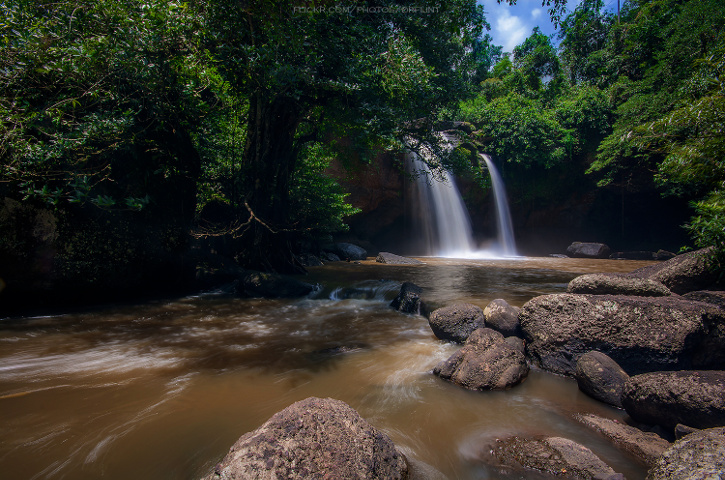
\includegraphics[width=0.49\linewidth]{./images/examples/subfloat-example-01.jpg}%
	}%
	\hfill%
	\subfloat[Bangkok, Thailand (\copyright\ Prachanart Viriyaraks)]{%
		\label{fig:subfloat-example-02}%
		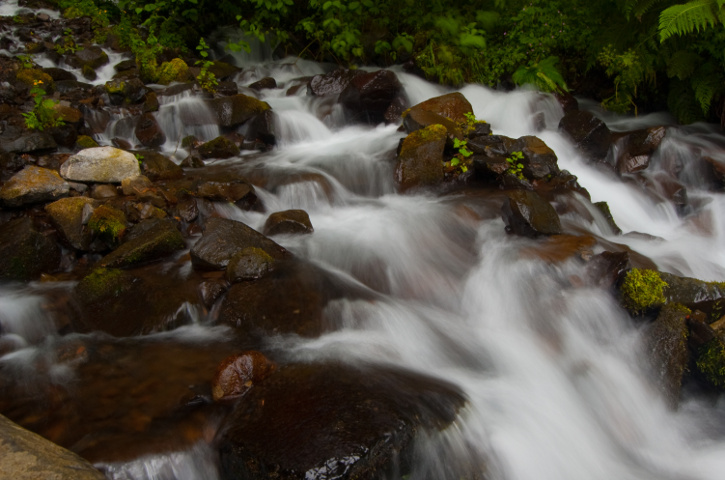
\includegraphics[width=0.49\linewidth]{./images/examples/subfloat-example-02.jpg}%
	}%
	\\%
	\subfloat[Wahkeena Falls, Lincoln Park, USA (\copyright\ srslyguys)]{%
		\label{fig:subfloat-example-03}%
		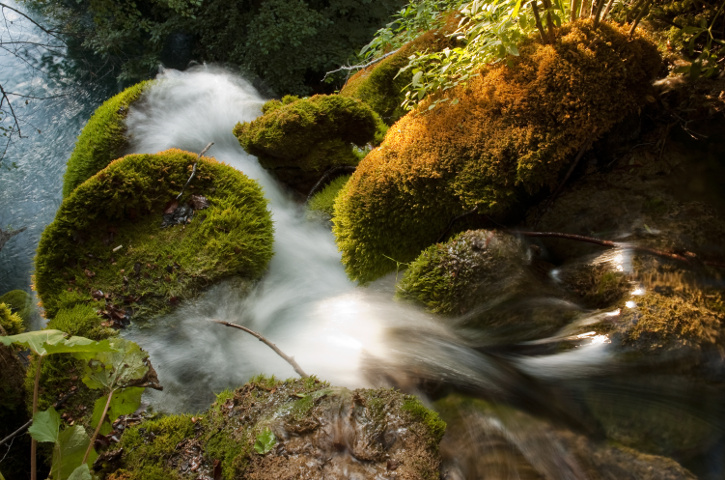
\includegraphics[width=0.49\linewidth]{./images/examples/subfloat-example-03.jpg}%
	}%
	\hfill%
	\subfloat[Nacionalni park Plitvička jezer, Kroatien (\copyright\ Roman Bonnefoy)]{%
		\label{fig:subfloat-example-04}%
		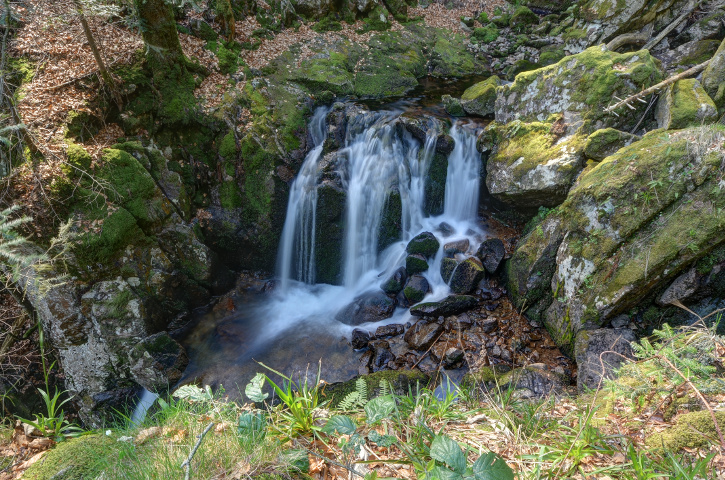
\includegraphics[width=0.49\linewidth]{./images/examples/subfloat-example-04.jpg}%
	}%
	\caption[Bild mit Unterabbildungen]{Wasserfälle der Welt als Beispiel für Unterabbildungen}%
	\label{fig:subfloat-example}%
\end{figure}

Der Beispielcode dafür ist in \cref{lst:subfigures} dargestellt.

\begin{latex}[caption={Unterabbildungen in LaTeX},label={lst:subfigures}]
\begin{figure}[h]%
	\centering%
	\subfloat[Unterbezeichnung 1)]{%
		\label{fig:UnterAbb1}%
		\includegraphics[width=0.49\linewidth]{Bildpfad/Bild1}%
	}%
	\hfill%
	\subfloat[Unterbezeichnung 2]{%
		\label{fig:UnterAbb2}%
		\includegraphics[width=0.49\linewidth]{Bildpfad/Bild2}%
	}%
	\\%
	\subfloat[Unterbezeichnung 3)]{%
		\label{fig:UnterAbb3}%
		\includegraphics[width=0.49\linewidth]{Bildpfad/Bild3}%
	}%
	\hfill%
	\subfloat[Unterbezeichnung 4]{%
		\label{UnterAbb4}%
		\includegraphics[width=0.49\linewidth]{Bildpfad/Bild4}%
	}%
\caption[Kurzversion]{Langversion der Bildunterschrift}%
\label{fig:MeinGanzesBild}%
\end{figure}
\end{latex}

Man beachte die abschließenden Prozent-Zeichen am Ende jeder Zeile!

%%%%%%%%%%%%%%%%%%%%%%%%%%%%%%%%%%%%%%%%%%%%%%%%%%%%%%%%%%%%
\subsection[TikZ-Grafiken]{\index{TikZ}\index{Bild!TikZ}\gls{gls:tikz}-Grafiken}%
\label{sec:TikZ}
%%%%%%%%%%%%%%%%%%%%%%%%%%%%%%%%%%%%%%%%%%%%%%%%%%%%%%%%%%%%
%
\Gls{gls:tikz} eignet sich hervorragend, um wissenschaftliche Zeichnungen,
Vektorgrafiken und \index{Diagramm}Diagramme direkt mithilfe von LaTeX
zu setzen, sodass die Schrift direkt zum restlichen Dokument passt.
Zu dem \pkg{tikz}-\gls{gls:pkg} und dem darauf aufsetzenden \pkg{PGFplots}-\gls{gls:pkg} gibt
es hervorragende Dokumentation \parencites{Tantau2013}{Feuersaenger2014}.
Mit \gls{gls:tikz} und \gls{gls:pgfplots} lassen sich viele gute Sachen machen.


Der Code für die Einbindung einer \gls{gls:tikz}-Grafik sieht folgendermaßen aus:
\begin{latex}[caption={Einbindung einer TikZ-Zeichnung in LaTeX},label={lst:tikz-figure}]
\begin{figure}[h]%
  \centering%
  \tikzsetnextfilename{TikZ-Bild}%
  \resizebox{\textwidth}{!}{%   <--- optionale Skalierung
    \input{./figures-src/TikZ-Bild.tex}%
  }%                            <--- optionale Skalierung
  \caption[Kurzversion für das Abbildungsverzeichnis]{%
           Eine tolle sehr lange Abbildungsunterschrift}%
  \label{fig:my-tikz-figure}%
\end{figure}
\end{latex}

Eine Skalierung auf die volle Seitenbreite oder ein vielfaches davon im Falle von Unterabbildungen kann bei Bedarf mit Hilfe der Anweisung
\texttt{\bs resizebox\{\bs textwidth\}\{!\}\{...\}}
durchgeführt werden.

Das Kommando \verb+\tikzsetnextfilename{...}+ ist nicht unbedingt notwendig,
 aber sehr zu empfehlen, da dies als Name für das temporäre Kompilat im Ordner
\printfilepath{./figures-compiled/} genommen wird.
Dieser sollte gleich dem Namen des Quelldatei (ohne Endung) gewählt werden.
Ansonsten nimmt \texttt{pdflatex} eine hochlaufende Nummer als Dateiname,
was die Fehlersuche sehr erschwert.

Nachfolgend finden sich einige Beispiele für TikZ-Zeichnungen, nämlich
eine Übersicht über die KIT-Corporate-Identity-Farben (\cref{fig:kit-colors}),
ein kommutatives Diagramm (\cref{fig:kpca}),
ein Netzwerkkommunikationsgraph (\cref{fig:net-comm}),
einfache \index{Diagramm!Punkt-}Punktdiagramme (\cref{fig:ica})
und etwas aufwendigere Diagramme mit mehreren
\index{Achsensystem|see{Diagramm}}Achsensystemen (\cref{fig:pca}).

Vorzugsweise sollten für die Grafiken die KIT-Corporate-Identity-Farben verwendet werden,
die sowohl eine RGB"=Definition für die Darstellung online,
als auch eine CMYK"=Definition für den Offset-Druck haben.%
\footnote{Bei Erstellung der Manuskriptversionen
für die Online-Veröffentlichung bzw. für den Offset-Druck
ist auf die korrekte Einstellung der Option \printkeyword{useCMYKcolors}
in der Datei \printfilepath{preambel/AlleAngaben.tex} zu achten
(\printkeyword{false} für die Online-Veröffentlichung und \printkeyword{true} für den Druck!}

\begin{figure}[hp]%
	\centering%
  \tikzsetnextfilename{kit-colors}%
	%\resizebox{\textwidth}{!}{%
		\begin{tikzpicture}[
box/.append style={rectangle,inner sep=0pt,outer sep=0pt,minimum size=1.5em,draw=none,fill=#1},
label/.style={font={\ttfamily\footnotesize},anchor=east},
caption/.style={font={\ttfamily\footnotesize},rotate=90,anchor=west}
]
\matrix[row sep=.2em,column sep=.2em] {
  &
\node[caption] {\textbackslash{}KITgreen...};      &
\node[caption] {\textbackslash{}KITblue...};       &
\node[caption] {\textbackslash{}KITblack...};      &
\node[caption] {\textbackslash{}KITpalegreen...};  &
\node[caption] {\textbackslash{}KITyellow...};     &
\node[caption] {\textbackslash{}KITorange...};     &
\node[caption] {\textbackslash{}KITbrown...};      &
\node[caption] {\textbackslash{}KITred...};        &
\node[caption] {\textbackslash{}KITlilac...};      &
\node[caption] {\textbackslash{}KITcyanblue...};   \\
\node[label] {};               &
\node[box=KITgreen      ] {};  &
\node[box=KITblue       ] {};  &
\node[box=KITblack      ] {};  &
\node[box=KITpalegreen  ] {};  &
\node[box=KITyellow     ] {};  &
\node[box=KITorange     ] {};  &
\node[box=KITbrown      ] {};  &
\node[box=KITred        ] {};  &
\node[box=KITlilac      ] {};  &
\node[box=KITcyanblue   ] {};  \\
\node[label] {...70};      &
\node[box=KITgreen70    ] {};  &
\node[box=KITblue70     ] {};  &
\node[box=KITblack70    ] {};  &
\node[box=KITpalegreen70] {};  &
\node[box=KITyellow70   ] {};  &
\node[box=KITorange70   ] {};  &
\node[box=KITbrown70    ] {};  &
\node[box=KITred70      ] {};  &
\node[box=KITlilac70    ] {};  &
\node[box=KITcyanblue70 ] {};  \\
\node[label] {...50};      &
\node[box=KITgreen50    ] {};  &
\node[box=KITblue50     ] {};  &
\node[box=KITblack50    ] {};  &
\node[box=KITpalegreen50] {};  &
\node[box=KITyellow50   ] {};  &
\node[box=KITorange50   ] {};  &
\node[box=KITbrown50    ] {};  &
\node[box=KITred50      ] {};  &
\node[box=KITlilac50    ] {};  &
\node[box=KITcyanblue50 ] {};  \\
\node[label] {...30};      &
\node[box=KITgreen30    ] {};  &
\node[box=KITblue30     ] {};  &
\node[box=KITblack30    ] {};  &
\node[box=KITpalegreen30] {};  &
\node[box=KITyellow30   ] {};  &
\node[box=KITorange30   ] {};  &
\node[box=KITbrown30    ] {};  &
\node[box=KITred30      ] {};  &
\node[box=KITlilac30    ] {};  &
\node[box=KITcyanblue30 ] {};  \\
\node[label] {...15};      &
\node[box=KITgreen15    ] {};  &
\node[box=KITblue15     ] {};  &
\node[box=KITblack15    ] {};  &
\node[box=KITpalegreen15] {};  &
\node[box=KITyellow15   ] {};  &
\node[box=KITorange15   ] {};  &
\node[box=KITbrown15    ] {};  &
\node[box=KITred15      ] {};  &
\node[box=KITlilac15    ] {};  &
\node[box=KITcyanblue15 ] {};  \\
};

\end{tikzpicture}%
	%}%
	\caption{KIT-Corporate-Identity-Farben}%
  \label{fig:kit-colors}%
\end{figure}

\begin{figure}[hp]%
	\centering%
  \tikzsetnextfilename{kpca}%
	%\resizebox{\textwidth}{!}{%
		\begin{tikzpicture}
\node (M) at (0,0) {$M$};
\node (F) [right=5em of M] {$F$};
\node (N) [right=5em of F] {$M'$};

\draw[-latex] (M)--(F) node[above,midway,font=\scriptsize] {$\varphi$};
\draw[-latex] (F)--(N) node[above,midway,font=\scriptsize] {PCA};
\draw[-latex,dotted] (M) to[bend left] node[above,midway,font=\scriptsize] {kernelized PCA} (N);

\node[below=3ex of M,font=\scriptsize] {$\dim(M) = d$};
\node[below=3ex of F,font=\scriptsize] {$\dim(F) \gg d$};
\node[below=3ex of N,font=\scriptsize] {$\dim(M') = d' < d$};
\end{tikzpicture}%
	%}%
	\caption{Kommutative Diagramm mit TikZ}%
  \label{fig:kpca}%
\end{figure}

\begin{figure}[hp]%
	\centering
  \tikzsetnextfilename{net-comm}%
	\resizebox{\textwidth}{!}{%
		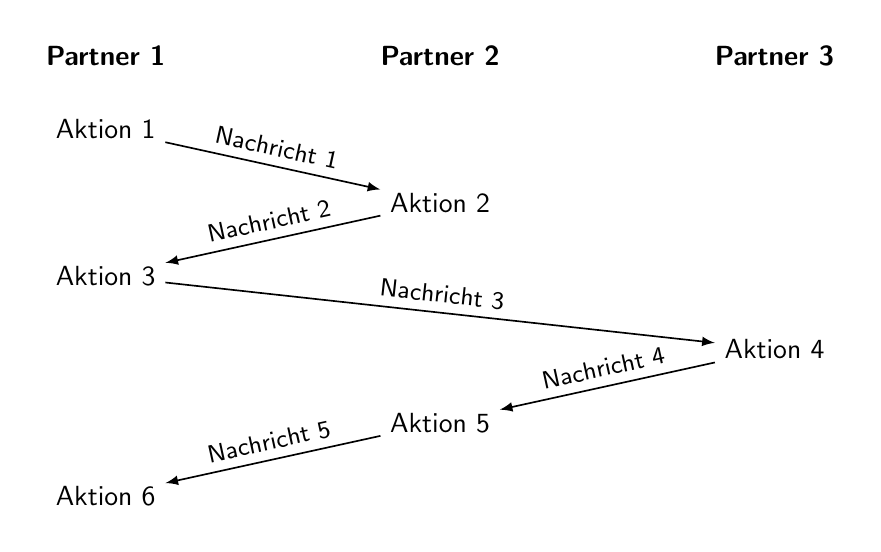
\begin{tikzpicture}[
every node/.append style={font={\sffamily}},
caption/.append style={font={\sffamily\bfseries}},
comm/.style={-latex,semithick},
msg/.style={midway,sloped,above,font={\sffamily\small}},
]
\matrix[row sep=3ex,column sep=25mm] {
\node[caption] {Partner 1};  & \node[caption] {Partner 2}; & \node[caption] {Partner 3}; \\
\node (A1) {Aktion 1}; & & \\
& \node (A2) {Aktion 2}; & \\
\node (A3) {Aktion 3}; & & \\
& & \node (A4) {Aktion 4};\\
& \node (A5) {Aktion 5}; & \\
\node (A6) {Aktion 6}; & & \\
};

\draw[comm] (A1)--(A2) node[msg] {Nachricht 1};
\draw[comm] (A2)--(A3) node[msg] {Nachricht 2};
\draw[comm] (A3)--(A4) node[msg] {Nachricht 3};
\draw[comm] (A4)--(A5) node[msg] {Nachricht 4};
\draw[comm] (A5)--(A6) node[msg] {Nachricht 5};

\end{tikzpicture}%
	}%
	\caption{Netzwerkkommunikationsgraph mit TikZ}%
  \label{fig:net-comm}%
\end{figure}

\begin{figure}[hp]%
	\centering%
	\subfloat[Ursprünglicher Merkmalsraum]{%
		\label{fig:ica-1}%
		\tikzsetnextfilename{ica-1}%
		\resizebox{0.45\textwidth}{!}{%
			\begin{tikzpicture}[
my_plot/.style={draw=none,every mark/.append style={draw=KITblue,fill=KITblue},mark=*,mark size=1.5pt},
]

\begin{axis}[
width=4cm,
height=4cm,
xmin = -1.1,
xmax = 1.1,
xlabel={$m_1$},
ymin = -1.1,
ymax = 1.1,
ylabel={$m_2$},
axis lines=center,
scale only axis,
]

\addplot[my_plot] coordinates {
(0.030,-0.062) (-0.118,-0.004) (0.276,0.236) (0.578,0.566) (-0.143,-0.014)
(0.304,0.257) (0.423,0.535) (0.205,0.344) (0.364,0.365) (-0.327,-0.368)
(0.176,0.310) (-0.298,-0.360) (0.153,0.279) (0.010,0.062) (0.150,0.231)
(-0.301,-0.214) (0.079,0.094) (-0.241,-0.161) (-0.474,-0.461) (0.091,0.173)
(0.541,0.601) (-0.288,-0.153) (0.013,-0.093) (0.290,0.115) (0.194,0.028)
(0.486,0.370) (0.201,0.227) (0.510,0.510) (-0.211,-0.293) (-0.058,0.088)
(0.326,0.176) (-0.591,-0.574) (0.071,0.204) (-0.401,-0.308) (0.206,0.111)
(-0.529,-0.667) (0.064,0.040) (0.032,0.035) (-0.349,-0.291) (0.476,0.316)
(0.625,0.624) (0.312,0.234) (0.076,-0.079) (0.016,0.018) (-0.556,-0.655)
(-0.308,-0.217) (0.248,0.122) (-0.515,-0.428) (-0.121,0.041) (0.260,0.228)
(-0.317,-0.406) (0.650,0.483) (-0.198,-0.097) (-0.427,-0.495) (0.429,0.553)
(-0.432,-0.538) (-0.460,-0.440) (-0.558,-0.654) (0.516,0.586) (-0.230,-0.205)
(0.148,0.199) (-0.417,-0.240) (-0.138,-0.040) (-0.252,-0.403) (0.096,0.010)
(-0.478,-0.339) (0.628,0.650) (0.054,-0.104) (0.502,0.429) (0.051,0.045)
(0.099,0.106) (0.344,0.214) (-0.359,-0.334) (0.291,0.187) (0.176,0.217)
(0.329,0.362) (-0.270,-0.116) (-0.136,-0.008) (-0.446,-0.533) (0.653,0.585)
(0.474,0.540) (0.093,0.136) (0.356,0.473) (0.232,0.217) (0.592,0.659)
(-0.326,-0.170) (-0.683,-0.497) (-0.484,-0.357) (-0.607,-0.635) (-0.044,-0.041)
(-0.681,-0.533) (-0.306,-0.401) (0.189,0.334) (0.420,0.259) (0.040,0.086)
(-0.148,-0.303) (-0.585,-0.507) (0.424,0.330) (0.597,0.688) (0.211,0.271)
(-0.429,-0.360) (0.280,0.188) (0.375,0.252) (-0.505,-0.528) (-0.064,-0.043)
(-0.257,-0.140) (0.302,0.262) (-0.228,-0.293) (0.154,0.122) (-0.549,-0.403)
(0.034,-0.027) (0.207,0.122) (-0.538,-0.648) (-0.601,-0.664) (-0.623,-0.433)
(-0.552,-0.417) (-0.094,-0.166) (0.469,0.496) (0.580,0.497) (0.212,0.159)
(0.515,0.627) (-0.070,-0.167) (-0.101,-0.015) (-0.244,-0.328) (-0.372,-0.477)
(0.256,0.199) (-0.607,-0.560) (-0.462,-0.554) (0.132,0.086) (0.066,0.050)
(0.230,0.157) (-0.502,-0.556) (0.666,0.490) (0.407,0.425) (-0.219,-0.355)
(-0.250,-0.285) (0.266,0.159) (-0.263,-0.412) (0.028,0.091) (-0.086,0.043)
(-0.633,-0.504) (-0.420,-0.399) (0.378,0.380) (-0.008,-0.163) (-0.226,-0.278)
(0.148,0.193) (-0.629,-0.582) (0.586,0.450) (0.025,0.136) (-0.445,-0.360)
};

\end{axis}
\end{tikzpicture}
		}%
	}%
	\hfill%
	\subfloat[Transienter Merkmalsraum (Nach Whitening, z.\,B. durch \gls{ac:PCA} inkl. Normalisierung)]{%
		\label{fig:ica-2}%
		\tikzsetnextfilename{ica-2}%
		\resizebox{0.45\textwidth}{!}{%
			\begin{tikzpicture}[
my_plot/.style={draw=none,every mark/.append style={draw=KITblue,fill=KITblue},mark=*,mark size=1.5pt},
]

\begin{axis}[
width=4cm,
height=4cm,
xmin = -1.1,
xmax = 1.1,
xlabel={$m'_1$},
ymin = -1.1,
ymax = 1.1,
ylabel={$m'_2$},
axis lines=center,
scale only axis,
]

\addplot[my_plot] coordinates {
(-0.273,-0.278) (0.267,0.398) (0.117,-0.289) (0.483,-0.399) (0.293,0.455)
(0.120,-0.326) (0.747,0.049) (0.640,0.265) (0.329,-0.231) (-0.430,0.090)
(0.597,0.269) (-0.471,0.014) (0.549,0.259) (0.180,0.141) (0.401,0.136)
(0.014,0.439) (0.120,-0.008) (0.044,0.379) (-0.384,0.338) (0.349,0.173)
(0.681,-0.175) (0.183,0.566) (-0.335,-0.309) (-0.310,-0.678) (-0.368,-0.593)
(0.057,-0.637) (0.266,-0.054) (0.457,-0.325) (-0.457,-0.098) (0.425,0.450)
(-0.196,-0.631) (-0.474,0.426) (0.500,0.334) (-0.059,0.516) (-0.127,-0.402)
(-0.926,-0.054) (-0.019,-0.107) (0.038,-0.012) (-0.122,0.388) (-0.094,-0.754)
(0.560,-0.398) (0.026,-0.418) (-0.439,-0.488) (0.021,-0.004) (-0.822,0.075)
(0.020,0.454) (-0.190,-0.516) (-0.180,0.573) (0.420,0.535) (0.130,-0.255)
(-0.575,-0.050) (0.039,-0.885) (0.151,0.410) (-0.607,0.078) (0.790,0.077)
(-0.736,-0.026) (-0.348,0.349) (-0.817,0.082) (0.692,-0.130) (-0.126,0.216)
(0.301,0.052) (0.202,0.765) (0.195,0.363) (-0.719,-0.267) (-0.195,-0.306)
(0.024,0.696) (0.635,-0.338) (-0.469,-0.483) (0.215,-0.523) (0.028,-0.048)
(0.113,-0.042) (-0.116,-0.587) (-0.242,0.298) (-0.078,-0.479) (0.291,0.003)
(0.405,-0.114) (0.259,0.605) (0.297,0.450) (-0.684,0.038) (0.365,-0.607)
(0.644,-0.112) (0.223,0.062) (0.701,0.104) (0.158,-0.192) (0.752,-0.185)
(0.214,0.646) (-0.007,0.960) (-0.020,0.667) (-0.635,0.308) (-0.029,0.037)
(-0.131,0.849) (-0.587,-0.076) (0.645,0.292) (-0.150,-0.724) (0.184,0.102)
(-0.638,-0.344) (-0.270,0.594) (0.073,-0.536) (0.833,-0.122) (0.385,0.036)
(-0.160,0.468) (-0.048,-0.437) (-0.065,-0.586) (-0.531,0.254) (0.010,0.099)
(0.151,0.495) (0.141,-0.305) (-0.417,-0.039) (0.033,-0.188) (-0.016,0.763)
(-0.166,-0.191) (-0.093,-0.373) (-0.843,0.031) (-0.746,0.204) (0.060,0.933)
(-0.055,0.733) (-0.320,-0.144) (0.510,-0.221) (0.252,-0.601) (0.018,-0.283)
(0.829,-0.011) (-0.381,-0.230) (0.190,0.308) (-0.492,-0.081) (-0.679,-0.062)
(0.042,-0.326) (-0.391,0.520) (-0.717,0.032) (-0.032,-0.214) (0.009,-0.085)
(-0.034,-0.355) (-0.627,0.168) (0.022,-0.923) (0.424,-0.209) (-0.641,-0.245)
(-0.339,0.060) (-0.110,-0.472) (-0.722,-0.253) (0.230,0.160) (0.345,0.421)
(-0.147,0.768) (-0.309,0.326) (0.348,-0.233) (-0.513,-0.434) (-0.372,-0.002)
(0.278,0.031) (-0.413,0.531) (0.082,-0.757) (0.384,0.297) (-0.122,0.523)
};

\end{axis}
\end{tikzpicture}%
		}%
	}%
	\hfill%
	\subfloat[Transformierter Merkmalsraum]{%
		\label{fig:ica-3}%
		\tikzsetnextfilename{ica-3}%
		\resizebox{0.45\textwidth}{!}{%
			\begin{tikzpicture}[
my_plot/.style={draw=none,every mark/.append style={draw=KITblue,fill=KITblue},mark=*,mark size=1.5pt},
]

\begin{axis}[
width=4cm,
height=4cm,
xmin = -1.1,
xmax = 1.1,
xlabel={$m''_1$},
ymin = -1.1,
ymax = 1.1,
ylabel={$m''_2$},
axis lines=center,
scale only axis,
]

\addplot[my_plot] coordinates {
(-0.389,-0.004) (0.470,0.093) (-0.122,-0.287) (0.059,-0.623) (0.529,0.115)
(-0.146,-0.316) (0.563,-0.493) (0.640,-0.265) (0.069,-0.396) (-0.241,0.367)
(0.613,-0.232) (-0.323,0.342) (0.572,-0.205) (0.227,-0.027) (0.379,-0.188)
(0.320,0.300) (0.079,-0.090) (0.299,0.237) (-0.033,0.510) (0.369,-0.124)
(0.358,-0.605) (0.530,0.271) (-0.455,0.019) (-0.699,-0.260) (-0.680,-0.159)
(-0.410,-0.491) (0.150,-0.226) (0.093,-0.554) (-0.393,0.254) (0.619,0.017)
(-0.584,-0.307) (-0.034,0.636) (0.590,-0.118) (0.323,0.406) (-0.374,-0.194)
(-0.693,0.617) (-0.089,-0.062) (0.018,-0.035) (0.188,0.361) (-0.600,-0.467)
(0.114,-0.678) (-0.277,-0.314) (-0.655,-0.035) (0.012,-0.018) (-0.528,0.634)
(0.335,0.306) (-0.499,-0.230) (0.278,0.532) (0.676,0.081) (-0.088,-0.272)
(-0.442,0.371) (-0.599,-0.654) (0.397,0.183) (-0.374,0.484) (0.613,-0.504)
(-0.539,0.502) (0.001,0.493) (-0.520,0.635) (0.398,-0.581) (0.063,0.242)
(0.249,-0.176) (0.684,0.398) (0.395,0.119) (-0.697,0.320) (-0.354,-0.078)
(0.509,0.475) (0.210,-0.688) (-0.674,-0.010) (-0.218,-0.522) (-0.014,-0.053)
(0.050,-0.110) (-0.498,-0.333) (0.040,0.382) (-0.394,-0.284) (0.208,-0.204)
(0.206,-0.367) (0.611,0.245) (0.528,0.108) (-0.457,0.510) (-0.171,-0.688)
(0.376,-0.535) (0.202,-0.114) (0.569,-0.422) (-0.024,-0.247) (0.401,-0.663)
(0.608,0.305) (0.674,0.684) (0.457,0.486) (-0.231,0.667) (0.005,0.047)
(0.508,0.693) (-0.469,0.362) (0.663,-0.250) (-0.618,-0.406) (0.203,-0.058)
(-0.694,0.208) (0.229,0.611) (-0.327,-0.431) (0.503,-0.676) (0.298,-0.247)
(0.217,0.444) (-0.343,-0.275) (-0.460,-0.368) (-0.196,0.555) (0.077,0.063)
(0.457,0.243) (-0.116,-0.315) (-0.322,0.267) (-0.110,-0.157) (0.528,0.550)
(-0.253,-0.018) (-0.329,-0.198) (-0.574,0.618) (-0.384,0.672) (0.702,0.617)
(0.480,0.557) (-0.329,0.124) (0.205,-0.517) (-0.247,-0.604) (-0.188,-0.213)
(0.578,-0.594) (-0.432,0.106) (0.352,0.083) (-0.406,0.291) (-0.523,0.436)
(-0.201,-0.260) (0.091,0.644) (-0.484,0.530) (-0.173,-0.129) (-0.054,-0.067)
(-0.275,-0.227) (-0.325,0.562) (-0.637,-0.668) (0.152,-0.447) (-0.626,0.280)
(-0.197,0.283) (-0.411,-0.256) (-0.690,0.332) (0.276,-0.050) (0.542,0.054)
(0.439,0.647) (0.012,0.449) (0.081,-0.411) (-0.670,0.056) (-0.265,0.262)
(0.218,-0.175) (0.083,0.668) (-0.477,-0.594) (0.482,-0.061) (0.284,0.456)
};

\end{axis}
\end{tikzpicture}%
		}%
}%
\caption{Diagramme mit TikZ direkt in LaTeX (hier: Die Schritte der \enquote{Independent component analysis})}%
\label{fig:ica}%
\end{figure}

\begin{figure}[hp]
	\centering%
	\subfloat[Ungünstige Projektion]{%
		\label{fig:pca-1}%
		\tikzsetnextfilename{pca-1}%
		\resizebox{0.48\textwidth}{!}{%
			\begin{tikzpicture}[
my_plot_1/.style={draw=none,every mark/.append style={draw=KITblue,fill=KITblue},mark=*},
my_plot_2/.style={draw=none,every mark/.append style={draw=KITred,fill=KITred},mark=*},
trans_arrow/.style={semithick,KITorange,-latex},
]

\begin{axis}[
width=4cm,
height=4cm,
xmin = -0.2,
xmax = 2.3,
xlabel={$m_1$},
ymin = -0.2,
ymax = 2.3,
ylabel={$m_2$},
xticklabel=\empty,
yticklabel=\empty,
axis lines=center,
clip=false,
scale only axis,
]

\addplot[my_plot_1] coordinates {
(1.3,0.38)
(1.42,0.71)
(1.48,0.60)
(1.64,0.54)
(1.65,0.81)
(1.68,0.89)
(1.79,1.11)
(1.88,1.18)
(1.89,1.46)
(1.94,1.35)
(1.86,1.65)
(2.02,1.83)
(2.12,1.83)
(2.19,2.26)
(2.21,2.07)
};

\addplot[my_plot_2] coordinates {
(1.28,0.58)
(1.33,0.93)
(1.54,1.03)
(1.54,1.26)
(1.51,1.41)
(1.72,1.52)
(1.76,1.87)
(1.80,1.90)
(1.90,2.00)
(1.91,2.27)
(2.05,2.40)
};

\coordinate(CoM) at (axis cs:1.71,1.38) {};

\draw[trans_arrow] (axis cs:0,0)--(CoM) node[midway,above left] {$m_0$};

\end{axis}

\begin{axis}[
width=5cm,
height=2.5cm,
xmin = -1.5,
xmax = 1.5,
xlabel={$m'_1$},
ymin = -0.75,
ymax = 0.75,
ylabel={$m'_2$},
axis lines=center,
xlabel style={anchor=north west},
ylabel style={anchor=south west},
xticklabel=\empty,
yticklabel=\empty,
clip=false,
anchor=origin,
at={(CoM)},
rotate around={65:(current axis.origin)},
clip=false,
scale only axis
]

\addplot+[my_plot_1] coordinates {
(-2,-0.0510)
(-2,-0.0203)
(-2,-0.1212)
(-2,-0.2916)
(-2,-0.1865)
(-2,-0.1799)
(-2,-0.1866)
(-2,-0.2386)
(-2,-0.1293)
(-2,-0.2211)
(-2,-0.0218)
(-2,-0.0908)
(-2,-0.1814)
(-2,-0.0631)
(-2,-0.1615)
};

\addplot+[my_plot_2] coordinates {
(-2,0.0516)
(-2,0.1542)
(-2,0.0062)
(-2,0.1034)
(-2,0.1939)
(-2,0.0501)
(-2,0.1618)
(-2,0.1382)
(-2,0.0898)
(-2,0.1949)
(-2,0.1229)
};

\draw[trans_arrow,shorten <=2pt,shorten >=3pt] (axis cs:-1.5,0)--(axis cs:-2,0) node[midway,right,font={\footnotesize},align=left] {Projektion\\auf $e_2$};
\draw[semithick] (axis cs:-2,-0.5)--(axis cs:-2,0.4);

\addplot+[my_plot_1] coordinates {
(-1.0796,-1.5)
(-0.7298,-1.5)
(-0.8041,-1.5)
(-0.7909,-1.5)
(-0.5420,-1.5)
(-0.4568,-1.5)
(-0.2109,-1.5)
(-0.1094,-1.5)
(0.1486,-1.5)
(0.0700,-1.5)
(0.3081,-1.5)
(0.5389,-1.5)
(0.5811,-1.5)
(1.0004,-1.5)
(0.8367,-1.5)
};

\addplot+[my_plot_2] coordinates {
(-0.9068,-1.5)
(-0.5684,-1.5)
(-0.3891,-1.5)
(-0.1806,-1.5)
(-0.0573,-1.5)
(0.1311,-1.5)
(0.4652,-1.5)
(0.5093,-1.5)
(0.6422,-1.5)
(0.8911,-1.5)
(1.0681,-1.5)
};

\draw[trans_arrow,shorten <=2pt,shorten >=3pt] (axis cs:0,-0.75)--(axis cs:0,-1.5) node[midway,anchor=north east,font={\footnotesize},align=left] {Projektion\\auf $e_1$};
\draw[semithick] (axis cs:-1.3,-1.5)--(axis cs:1.3,-1.5);

\end{axis}

\end{tikzpicture}%
		}%
	}\hfill%
	\subfloat[Zielführende Projektion]{%
		\label{fig:pca-2}%
		\tikzsetnextfilename{pca-2}%
		\resizebox{0.48\textwidth}{!}{%
			\begin{tikzpicture}[
my_plot_1/.style={draw=none,every mark/.append style={draw=KITblue,fill=KITblue},mark=*},
my_plot_2/.style={draw=none,every mark/.append style={draw=KITred,fill=KITred},mark=*},
trans_arrow/.style={semithick,KITorange,-latex},
]

\begin{axis}[
width=4cm,
height=4cm,
xmin = -0.2,
xmax = 2.3,
xlabel={$m_1$},
ymin = -0.2,
ymax = 2.3,
ylabel={$m_2$},
xticklabel=\empty,
yticklabel=\empty,
axis lines=center,
clip=false,
scale only axis,
]

\addplot[my_plot_1] coordinates {
(1.3,0.38)
(1.28,0.58)
(1.42,0.71)
(1.48,0.60)
(1.64,0.54)
(1.33,0.93)
(1.65,0.81)
(1.68,0.89)
(1.54,1.03)
(1.54,1.26)
(1.79,1.11)
(1.88,1.18)
(1.51,1.41)
};

\addplot[my_plot_2] coordinates {
(1.72,1.52)
(1.89,1.46)
(1.94,1.35)
(1.86,1.65)
(1.76,1.87)
(1.80,1.90)
(1.90,2.00)
(2.02,1.83)
(2.12,1.83)
(1.91,2.27)
(2.19,2.26)
(2.21,2.07)
(2.05,2.40)
};

\coordinate(CoM) at (axis cs:1.71,1.38) {};

\draw[trans_arrow] (axis cs:0,0)--(CoM) node[midway,above left] {$m_0$};

\end{axis}

\begin{axis}[
width=5cm,
height=2.5cm,
xmin = -1.5,
xmax = 1.5,
xlabel={$m'_1$},
ymin = -0.75,
ymax = 0.75,
ylabel={$m'_2$},
axis lines=center,
xlabel style={anchor=north west},
ylabel style={anchor=south west},
xticklabel=\empty,
yticklabel=\empty,
clip=false,
anchor=origin,
at={(CoM)},
rotate around={65:(current axis.origin)},
clip=false,
scale only axis
]

\addplot+[my_plot_1] coordinates {
(-2,-0.0510)
(-2,0.0516)
(-2,-0.0203)
(-2,-0.1212)
(-2,-0.2916)
(-2,0.1542)
(-2,-0.1865)
(-2,-0.1799)
(-2,0.0062)
(-2,0.1034)
(-2,-0.1866)
(-2,-0.2386)
(-2,0.1939)
};

\addplot+[my_plot_2] coordinates {
(-2,0.0501)
(-2,-0.1293)
(-2,-0.2211)
(-2,-0.0218)
(-2,0.1618)
(-2,0.1382)
(-2,0.0898)
(-2,-0.0908)
(-2,-0.1814)
(-2,0.1949)
(-2,-0.0631)
(-2,-0.1615)
(-2,0.1229)
};

\draw[trans_arrow,shorten <=2pt,shorten >=3pt] (axis cs:-1.5,0)--(axis cs:-2,0) node[midway,right,font={\footnotesize},align=left] {Projektion\\auf $e_2$};
\draw[semithick] (axis cs:-2,-0.5)--(axis cs:-2,0.4);

\addplot+[my_plot_1] coordinates {
(-1.0796,-1.5)
(-0.9068,-1.5)
(-0.7298,-1.5)
(-0.8041,-1.5)
(-0.7909,-1.5)
(-0.5684,-1.5)
(-0.5420,-1.5)
(-0.4568,-1.5)
(-0.3891,-1.5)
(-0.1806,-1.5)
(-0.2109,-1.5)
(-0.1094,-1.5)
(-0.0573,-1.5)
};

\addplot+[my_plot_2] coordinates {
(0.1311,-1.5)
(0.1486,-1.5)
(0.0700,-1.5)
(0.3081,-1.5)
(0.4652,-1.5)
(0.5093,-1.5)
(0.6422,-1.5)
(0.5389,-1.5)
(0.5811,-1.5)
(0.8911,-1.5)
(1.0004,-1.5)
(0.8367,-1.5)
(1.0681,-1.5)
};

\draw[trans_arrow,shorten <=2pt,shorten >=3pt] (axis cs:0,-0.75)--(axis cs:0,-1.5) node[midway,anchor=north east,font={\footnotesize},align=left] {Projektion\\auf $e_1$};
\draw[semithick] (axis cs:-1.3,-1.5)--(axis cs:1.3,-1.5);

\end{axis}

\end{tikzpicture}%
		}%
	}%
	\caption{Aufwändiges Diagramm mit TikZ (hier: Probleme der \enquote{Principal component analysis})}%
	\label{fig:pca}%
\end{figure}
%%%%%%%%%%%%%%%%%%%%%%%%%%%%%%%%%%%%%%%%%%%%%%%%%%%%%%%%%%%%
\section{Tabellen}%
\label{sec:Tabellen}
%%%%%%%%%%%%%%%%%%%%%%%%%%%%%%%%%%%%%%%%%%%%%%%%%%%%%%%%%%%%
Für eine ausführliche Erläuterung auch über gute und schlechte Tabellen
und deren Gestaltung empfiehlt sich die Lektüre des entsprechenden Artikels im \LaTeX{}"=Kompendium auf Wikibooks%
\footnote{\url{https://de.wikibooks.org/wiki/LaTeX-Kompendium:_Tabellen}}
sowie die Dokumentation des \pkg{booktabs}-Pakets \cite{Fear2005}.
\Ua stellt dieses Paket die Befehle
\begin{itemize*}
	\item \lstinline|\toprule|
	\item \lstinline|\midrule|
	\item \lstinline|\bottomrule|
\end{itemize*}
zur Verfügung.

Eine einfache Tabelle hat den folgenden Code:

\begin{latex}[caption={Einfache Tabelle in \LaTeX},label={lst:tabellenbeispiel}]
\begin{table}%
	\centering%
	\begin{tabularx}{\columnwidth}{l l X}%
		\toprule%
		Datei       &  Bedeutung    &  Benutzerinteraktion \\%
		\midrule%
		Diss.tex  &  Hauptdatei   &  nein     \\%
		images/   &  Bilder       &  ja       \\%
		content/  &  Kapitel      &  ja       \\%
		\bottomrule%
	\end{tabularx}%
	\caption{Dateien der Vorlage}%
	\label{tab:tabellenbeispiel}%
\end{table}
\end{latex}

Das Ergebnis sieht man in \cref{tab:tabellenbeispiel}.

\begin{table}%
	\centering%
	\begin{tabular}{l l l}%
		\toprule%
		Datei       &  Bedeutung    &  Benutzerinteraktion \\%
		\midrule%
		Diss.tex  &  Hauptdatei   &  nein     \\%
		images/   &  Bilder       &  ja       \\%
		content/  &  Kapitel      &  ja       \\%
		\bottomrule%
	\end{tabular}%
	\caption{Dateien der Vorlage}%
	\label{tab:tabellenbeispiel}%
\end{table}

Etwas komplizierter wird es, wenn man eine Tabelle mit alternierender Farbe einfügen möchte (\cref{tab:AlternierendeZeilenfarben}).

\begin{table}
\caption{Tabelle mit alternierender Zeilenfarbe}%
\label{tab:AlternierendeZeilenfarben}%
	\tablestyle%
	\tablealtcolored%
	\begin{tabular}{*{2}{v{0.45\textwidth}}}
		\toprule%
		\tableheadcolor%
		\tableheadformat Tabellenkopf &	\tableheadformat Tabellenkopf
		\tabularnewline%
		\midrule%
		%% Zwischenkopf ---------------------------------------------
		\multicolumn{2}{>{\columncolor{tablesubheadcolor}}l}{\bfseries\color{KITblue} Zwischenkopf}%
		\tabularnewline%
		%%-----------------------------------------------------------
		Inhalt  & Inhalt \tabularnewline
		Inhalt  & Inhalt \tabularnewline
		Inhalt  & Inhalt \tabularnewline
		%% Zwischenkopf ---------------------------------------------
		\multicolumn{2}{>{\columncolor{tablesubheadcolor}}l}{\bfseries\color{KITgreen} Zwischenkopf}%
		\tabularnewline
		%%-----------------------------------------------------------
		Inhalt  & Inhalt \tabularnewline
		Inhalt  & Inhalt \tabularnewline
		\bottomrule%
	\end{tabular}%
\end{table}

%% ------------------------------------------------------------
Lange Tabellen, die umbrochen werden sollen, können mit
\lstinline|\LTXtable{\textwidth}{Datei}|
eingebunden werden, wobei die Tabelle in eine Datei ausgelagert werden muss.
Ein Beispiel dafür sieht man in \cref{tab:MehrseitigeTabelle}.

\IfDefined{LTXtable}{%
	%--Einstellungen für Tabellen ----------
	\colorlet{tablerowcolor}{gray!10.0}%
	\renewcommand\tableheadcolor{\rowcolor{tableheadcolor}}%
	\renewcommand\tablehead{%
			\tableheadfontsize%
			\sffamily\bfseries%
			\slshape%
			\color{black}%
	}%
	%---------------------------------------
	{
		\tablestyle%
		%\tablealtcolored
		\rowcolors{1}{tablerowcolor}{white!100}%
		 \LTXtable{\textwidth}{tables/LongTableExample.tex}%
	}%
} % End If 
%
%
%
Sollten eine Tabelle einmal so breit sein, dass sie nicht mehr horizontal auf
eine Seite passt, so ist es natürlich möglich, diese mithilfe des Pakets
\printkeyword{rotfloat} \parencite{Sommerfeldt2004} in eine
\printkeyword{sidewaystable} statt in eine \printkeyword{table}-Umgebung zu setzen.
Also so:
\begin{latex}[caption={Gedrehte Tabelle},label={lst:rotated-table}]
\begin{sidewaystable}
  \centering%
  \begin{tabular}{...}%
    ...
  \end{tabular}%
  \caption{Bezeichnung}%
  \label{Referenzmarke}%
\end{sidewaystable}%
\end{latex}

Das Ergebnis sieht man in \cref{tab:ex-sideways}.

%% Um 90° gedrehte Tabelle
%
\begin{sidewaystable}[p]
\scriptsize%
%\tiny
\centering%
\begin{tabular}{l M M M M M}%
\toprule%
\addlinespace[0pt]%
 & \multicolumn{5}{c}{\bfseries Level} \tabularnewline
 & \multicolumn{2}{c}{\bfseries Qualitative} & \multicolumn{3}{c}{\bfseries Quantitative} \tabularnewline
 & \bfseries\centering Nominal & \bfseries\centering Ordinal & \bfseries\centering Interval & \bfseries\centering Ratio & \bfseries\centering Absolute \tabularnewline \addlinespace[0pt]\midrule\addlinespace[0pt]
Empirical relation &
\begin{tabitemize}\item[$\sim$] Equivalence\end{tabitemize} &
\begin{tabitemize}\item[$\sim$] Equivalence\item[$\prec$] Ordering\end{tabitemize} &
\begin{tabitemize}\item[$\sim$] Equivalence\item[$\prec$] Ordering\end{tabitemize} &
\begin{tabitemize}\item[$\sim$] Equivalence\item[$\prec$] Ordering\strut\end{tabitemize} &
\begin{tabitemize}\item[$\sim$] Equivalence\item[$\prec$] Ordering\strut\end{tabitemize} \tabularnewline \midrule
Empirical operation &
 &
 &
\begin{tabitemize}\item[$\oplus$] Addition\end{tabitemize} &
\begin{tabitemize}\item[$\oplus$] Addition\item[$\otimes$] Multiplication\strut\end{tabitemize} &
\begin{tabitemize}\item[$\oplus$] Addition\item[$\otimes$] Multiplication\strut\end{tabitemize} \tabularnewline \midrule
Feasable transformation &
$m' = f( m )$ for $f$ bij.\strut &
$m' = f( m )$ for $f$ mon.\strut &
$m' = am + b$ for $a>0$\strut &
$m' = am$ for $a>0$\strut &
$m' = m$\strut \tabularnewline \midrule
Examples of features &
\begin{tabitemize}\item Telephone numbers\item Postal codes\item Gender\strut\end{tabitemize} &
\begin{tabitemize}\item Grades\item Degree of hardness\item Wind intensity\strut\end{tabitemize} &
\begin{tabitemize}\item Temperatur in F\textdegree\item Calendric time\item Geographic altitude\strut\end{tabitemize} &
\begin{tabitemize}\item Temperatur in K\item Mass\item Length\item Electric current\strut\end{tabitemize} &
\begin{tabitemize}\item Quantum numbers\item Error number\strut\end{tabitemize} \tabularnewline \midrule
Range of features &
\begin{tabitemize}\item Numbers\item Names\item Symbols\strut\end{tabitemize} &
Natural numbers &
Real numbers &
Real, positive numbers &
Natural numbers \tabularnewline \midrule
Expressiveness & low & \dots & \dots & \dots & high\strut \tabularnewline \addlinespace[0pt]
\bottomrule%
\end{tabular}%
\caption{Beispiel für eine breite, gedrehte Tabelle (hier: Taxonomie der Maßskalen)}%
\label{tab:ex-sideways}%
\end{sidewaystable}
%%%%%%%%%%%%%%%%%%%%%%%%%%%%%%%%%%%%%%%%%%%%%%%%%%%%%%%%%%%%
\section{Mathematische Sätze, Lemmas, Definitionen etc.}%
\label{sec:Theoreme}
%%%%%%%%%%%%%%%%%%%%%%%%%%%%%%%%%%%%%%%%%%%%%%%%%%%%%%%%%%%%
%
Für eine mathematische Ausarbeitung gibt es LaTeX-\glspl{gls:umgebung}, um
\index{Satz|see{Theorem}}\index{Theorem}Sätze (Theoreme), \index{Lemma|see{Theorem}}Lemma,
\index{Beispiel|see{Theorem}}Beispiele etc. im üblichen Stil von
Mathematik-Büchern zu setzen und zu referenzieren. Vordefiniert sind die
\glspl{gls:umgebung}
\begin{itemize*}
  \item \texttt{theorem} für Sätze
  \item \texttt{definition} für Definitionen
  \item \texttt{lemma} für Lemma
  \item \texttt{corollary} für Korollare
  \item \texttt{proposition} für Propositionen
\end{itemize*}
Die übliche Verwendung ist
\begin{latex}[caption={Beispiel für Theorem-Umgebungen},label={lst:ntheorem}]
\begin{theorem}[Optionaler Name]\label{thm:my-theorem}
...
\end{theorem}
\end{latex}
Weitere Informationen findet man in der Dokumentation zum \texttt{ntheorem}-Paket
\parencite{May2011}. Das Ganze sieht dann beispielsweise wie folgt aus.

\begin{theorem}[Theorem von Arthur Dent]
\label{thm:arthur-dent} Die Antwort auf die Frage nach dem Leben, dem Universum und den ganzen Rest ist 42.
\end{theorem}

\begin{definition}
\LaTeX{} ist eine von Leslie Lamport 1980 entwickelter Satz von Makros zur Erweiterung von \TeX.
\end{definition}

\begin{proposition}[Zweifelhafte Folgerung]
LaTeX ist schön. Beweis folgt unmittelbar aus \cref{thm:arthur-dent}.
\end{proposition}

%%%%%%%%%%%%%%%%%%%%%%%%%%%%%%%%%%%%%%%%%%%%%%%%%%%%%%%%%%%%
\section{Quellcode-Listings}%
\index{Listing!Gestaltungsstil}%
\label{sec:Listings}
%%%%%%%%%%%%%%%%%%%%%%%%%%%%%%%%%%%%%%%%%%%%%%%%%%%%%%%%%%%%
%
Zum Einbinden und formatieren von \index{Code|see{Listing}}Quellcode"=Beispielen
-- sog. \index{Listing}Listings -- wird das Paket \pkg{listings}
\parencite{Hoffmann2014} verwendet.
Das Hervorheben von \index{Schlusselwort@Schlüsselwort}Schlüsselwörtern
wird von LaTeX automatisch erledigt,
wenn die korrekte Sprache des Listings angegeben ist.
Dies geschieht mit Hilfe der Option \printkeyword{language}
oder durch die Angabe eines entsprechend definierten Gestaltungsstils.

Im Befehl \lstinline|\lstset{...}|,
welcher in der Datei \printfilepath{preambel/preambel.tex} zu finden ist,
kann man einen globalen Stil für alle Listings vorgeben
(welcher jedoch bei Bedarf im Einzelfall überrufen werden kann).
Aktuell ist der etwas weiter oben im Code mit dem Befehl
\lstinline|\lstdefinestyle{...}| vordefinierte Stil
\printkeyword{latex} als Standardgestaltungsstil ausgewählt.

Neben \printkeyword{latex} sind in der Datei \printfilepath{preambel/preambel.tex}
auch noch \printkeyword{java} und \printkeyword{C++} als Gestaltungsstile vordefiniert.
Bei Bedarf lassen sich dort weitere Stile definieren und auswählen.

Zur Vereinfachung der Einbindung wurden zusätzlich Umgebungen
\printkeyword{latex}, \printkeyword{java} und \printkeyword{C++}
vordefiniert, die im Code mit \lstinline|\begin{<name>}...\end{<name>}|
direkt verwendet werden können (s. \cref{lst:java-listing}).
%
So bewirkt beispielsweise
%
\begin{latex}[caption={Beispiel eines Listings in Java},label={lst:java-listing}]
\begin{java}[caption={A Java Hello-World example},%
             label={lst:hello-world}]
public class HelloWorld {
  public static void main( String[] args ) {
    System.out.println( "HelloWorld" );
  }
}
\end{java}
\end{latex}
%
das folgende Ergebnis:
%
\begin{C++}[caption={A Java Hello-World example},label={lst:hello-world}]
public class HelloWorld {
  public static void main( String[] args ) {
    System.out.println( "HelloWorld" );
  }
}
\end{C++}

Man beachte, dass anders als bei Abbildungen und Tabellen
die Bezeichnung (\texttt{caption}) und die Referenzmarke (\texttt{label})
nicht als gesonderte Befehle sondern als optionale Argumente übergeben werden.
Dies liegt daran, dass ein Listing in der Regel keine Fließumgebung ist,
sondern an der Stelle im Text erscheint, an der sie im Code auch steht.
Ferner folgt ein Listing den ganz normalen Seitenumbruchsregeln.
Das heißt, überlanger Code wird einfach umgebrochen. 
Um ein Listing zu einem Fließobjekt zu machen, muss das optionale Argument
\texttt{float=<tbp>} angegeben werden.
Die \index{Platzierung}Plazierungsangabe \enquote{\texttt{h}} für \enquote{hier}
ist nicht erlaubt. Denn dies ist das Standardverhalten ohne \texttt{float}.
%%%%%%%%%%%%%%%%%%%%%%%%%%%%%%%%%%%%%%%%%%%%%%%%%%%%%%%%%%%%
\section{Querverweise und Hyperlinks}%
\label{sec:Querverweise}
%%%%%%%%%%%%%%%%%%%%%%%%%%%%%%%%%%%%%%%%%%%%%%%%%%%%%%%%%%%%
%
Querverweise sollten nicht mit dem Befehl \lstinline|\ref{...}| gesetzt werden,
sondern mit \lstinline|\cref{...}| und verwandten Befehlen aus dem Paket
\pkg{cleveref} \cite{Cubitt2013}.
Diese Befehle haben den Vorteil nicht nur die Nummer zu referenzieren,
sondern auch den Typ mit anzugeben.
Hinzu kommt eine intelligente Verwendung der Pluralform und
\index{Sortierung}Sortierung bei Mehrfachaufzählungen auch unterschiedlichen Typs.
Will man \bspw auf zwei Abbildungen und eine Tabelle mit den Marken (\enquote{Labels})
%
\begin{itemize*}
\item \texttt{fig:subfloat-example}
\item \texttt{tab:files-dirs-of-template}
\item \texttt{fig:kit-colors}
\end{itemize*}
%
verweisen, so schreibt man einfach per Komma getrennt
%
\begin{latex}[caption={Cleveres Referenzieren mit \bs cref},label={lst:cref}]
\cref{fig:subfloat-example,
      tab:ex-sideways,
      fig:kit-colors}
\end{latex}
%
und erhält als Resultat
\enquote{\cref{fig:subfloat-example,tab:ex-sideways,fig:kit-colors}}.

\index{URL}\index{Internetadresse|see{URL}}Internetadressen werden in das Kommando \lstinline|\url{...}| eingefasst.
Außerdem besteht die Möglichkeit mit dem Befehl \lstinline|\href{<URL>}{Text}| eine Textstelle mit einem Hyperlink zu versehen.
%%%%%%%%%%%%%%%%%%%%%%%%%%%%%%%%%%%%%%%%%%%%%%%%%%%%%%%%%%%%
\section{Mathematik}%
\label{sec:Mathe}
%%%%%%%%%%%%%%%%%%%%%%%%%%%%%%%%%%%%%%%%%%%%%%%%%%%%%%%%%%%%
%
Grundsätzlich gilt, was in \parencites{ams1999a}{ams1999b} steht. In der Datei
\printfilepath{preambel/05-math.tex} sind eine Menge Kurzkommandos definiert, um eine
einheitliche Typografie von \index{Skalare}Skalaren, \index{Vektoren}Vektoren,
\index{Matrizen}Matrizen, \index{Zufallsvariablen}Zufallsvariablen etc.
zur vereinfachen. In diese Dateien einfach mal reinschauen, welche Kurzkommandos
es gibt.

Auf zwei besondere Kommandos wird näher eingegangen, weil dies häufig falsch
gemacht wird.
\begin{itemize}
  \item Für die Matrixtransponierte gibt es das Kommando \verb#\Tr#, also
	\verb#$A^{\Tr}$# liefert $A^{\Tr}$
	
	\item Bei \index{Integral}Integralen muss das \enquote{Differential-d} gemäß
	ISO in aufrechter Schrift als Operator gesetzt sein mit einem kleinen Abstand
	zum Integranden. Hierfür gibt es das spezielle Kommando \verb#\diff#. Also
	\begin{equation}
	 \int^1_0 x^2 d x = \frac{1}{3} \qquad \text{(falsche Typografie!)}
	\end{equation}
	ist falsch, während \verb#\int^1_0 x^2 \diff x = \frac{1}{3}# das Richtige
	liefert
	\begin{equation}
	 \int^1_0 x^2 \diff x = \frac{1}{3} \qquad \text{(richtige Typografie!)}
	\end{equation}
\end{itemize}

%%%%%%%%%%%%%%%%%%%%%%%%%%%%%%%%%%%%%%%%%%%%%%%%%%%%%%%%%%%%
\section{Abkürzungsverzeichnis, Stichwortverzeichnis (Index) und Glossar}%
\label{sec:Glossare}
%%%%%%%%%%%%%%%%%%%%%%%%%%%%%%%%%%%%%%%%%%%%%%%%%%%%%%%%%%%%
%
Die Vorlage unterstützt auch ein Stichwortverzeichnis und ein Glossar. Ein
Stichwortverzeichnis (oder Index) ist einfach nur eine alphabetisch sortierte
Liste von Begriffen mit einer Auflistung der \index{Fundstelle}Fundstellen
im Dokument. Ein Glossar ist eine alphabetisch sortierte Liste von Begriffen mit
\index{Erklarung@Erklärung}Erklärung.

Der Index wird erzeugt, indem im Quellcode der Befehl \verb#\index{Begriff}#
eingefügt wird. Wichtig, der Begriff selbst wird dadurch nicht gedruckt, sondern
muss noch einmal wiederholt werden, um auch gedruckt zu werden. Dieses Verhalten
ist beabsichtigt, sodass im Index immer nur die Grundform des Wortes verwendet
wird, aber im Text natürlich die richtige Deklination. Also:
\begin{latex}[caption={Beispiel für Index},label={lst:index}]
Die meisten Funktionen dieser \index{Vorlage}Vorlage, werden durch
\index{Paket}Standardpakete bereitgestellt.
\end{latex}
Obiges Beispiel erzeugt einen Indexeintrag für \enquote{Vorlage} der auf
\enquote{Vorlage} verweist und einen Eintrag \enquote{Paket} der auf 
\enquote{Standardpaket} verweist.

Um ein Glossar zu erzeugen, müssen die Glossarbegriffe zunächst definiert werden.
Dies geschieht in der Datei \texttt{./content/00-glossary-definitions.tex}.
Es gibt zwei Haupttypen von Glossarbegriffen: Abkürzungen (Akronyme) und allg.
Einträge (z.\,B. Fachtermini).

Abkürzungen werden mit
\begin{latex}[caption={Definition von Abkürzungen},label={lst:acro}]
\newacronym[%
  shortplural={AUen},%
  longplural={Abgasuntersuchungen}%
] {au}{AU}{Abgasuntersuchung}
\end{latex}
Die drei Hauptargumente sind in dieser Reihenfolge Marke, Abkürzung und
Ausschreibung. Optionale Argumente sind die kurze und lange Pluralform.

Allgemeine Glossarbegriffe werden mit
\begin{latex}[caption={Definition von allg. Glossareinträgen},label={lst:gls}]
\longnewglossaryentry{pkg}{%
  name={Paket},%
  plural={Pakete}}%
{%
  Hier folgt eine lange Definition, die auch mehr als einen
	Absatz beinhalten darf.
}
\end{latex}
erzeugt.

Im Text werden die Einträge durch den Befehl \verb#\gls{gls:Marke}# verwendet.
Der wesentliche Unterschied zwischen einer Abkürzung und einem allg.
Glossareintrag ist, dass bei Abkürzungen bei erstmaliger Verwendung die
Abkürzung gedruckt und die Langform in Klammer dahinter gesetzt wird.
Bei allg. Glossareinträgen wird einfach nur der Name gesetzt. Statt
\verb#\gls{gls:Marke}# gibt es noch viele weitere Befehle, um im Kontext des
umgebenen Textes die korrekte Pluralform, Großschreibung am Satzanfang, etc.
zu gewährleisten. Hierfür konsultiere man das Handbuch zum Paket \texttt{glossaries}
(Pluralform, sic!) \parencite{talbot2014}.

%%%%%%%%%%%%%%%%%%%%%%%%%%%%%%%%%%%%%%%%%%%%%%%%%%%%%%%%%%%%
\section{Randnotizen}%
\label{sec:Randnotizen}
%%%%%%%%%%%%%%%%%%%%%%%%%%%%%%%%%%%%%%%%%%%%%%%%%%%%%%%%%%%%
%
Randnotizen 
\marginnote{Ich bin eine überflüssige Randnotiz}%
werden mit dem Kommando \lc{partitle} gesetzt.
Diese eignet sich zum Beispiel um im Text Stellen zu kennzeichnen,
an denen man noch arbeiten sollte.
Da die Vorgaben des \glsgen{ac:KSP} für den Seitenlayout
einen sehr kleinen Randbereich vorsehen, der zudem nicht bedruckt werden darf,
werden keine Randnotizen in der endgültigen Version des Manuskriptes akzeptiert.
Die Randnotizen lassen sich bequem in der Hauptdatei ausschalten,
indem man \texttt{\bs showif\{showMarginNotes\}}
zu \texttt{\bs hideif\{showMarginNotes\}} ändert.
%%%%%%%%%%%%%%%%%%%%%%%%%%%%%%%%%%%%%%%%%%%%%%%%%%%%%%%%%%%%
\section[Anpassungen für den Druck]{Anpassungen für den Druck}%
\index{Druck}%
\label{sec:Druckanpassungen}
%%%%%%%%%%%%%%%%%%%%%%%%%%%%%%%%%%%%%%%%%%%%%%%%%%%%%%%%%%%%
%
Vor der Abgabe einer Druckversion an den KSP-Verlag sollte die korrekte Schaltersetzung in der Datei \printfilepath{./preambel/AlleSchalter.tex} nochmals geprüft werden.
Insbesondere sollte mit der Einstellung
\lstinline|\setUserDefinedBoolean{showFrame}{true}|
die Satzspiegel-Ränder angezeigt werden und so kontrolliert werden,
ob nichts hinausragt und ob Tabellen und Bilder die komplett verfügbare Breite ausfüllen.
Besonders sollte man dabei auch die Overfullbox- und Underfullbox"=Warnungen achten und diese beheben.
Danach sollte der Schalter wieder auf \printkeyword{false} umgestellt werden.

Bei Abbildungen, die am Anfang einer Seite stehen, ist dabei zu achten,
dass es keinen leeren Zwischenraum zwischen dem oberen Rand des Satzspiegels und der Abbildung gibt.
Normalerweise passiert dies durch die Einstellungen der Vorlage automatisch.
Falls doch noch ein leeres Raum entsteht, liegt dies zumeist daran, dass die Abbildung selbst weiße Ränder hat.
Bei Binärbildern können diese durch Setzen der Optionen
\printkeyword{clip=true} und \printkeyword{trim=<left> <lower> <right> <upper>}
im \printkeyword{includegraphics}-Befehl beschnitten werden, z.B. so:
\lstinline|\includegraphics[clip=true, trim={0cm 1cm 0cm 1cm}]{Bildpfad\Dateiname}|.

Mit den Einstellungen 
\lstinline|\setUserDefinedBoolean{coloredlistings}{false}| und 
\lstinline|\setUserDefinedBoolean{coloredlinks}{false}|
sollte dafür gesorgt werden, dass alle Quellcode-Listings sowie Querverweise und URL-Adressen,
die normalerweise farbig sind, für die Druckversion nicht farbig gesetzt werden
und so die Anzahl der farbig zu druckenden Seiten reduziert wird.

Schließlich kann mit der Einstellung
\lstinline|\setUserDefinedBoolean{useCMYKcolors}{true}|
eine Farbkonvertierung aller Farben in den CMYK-Farbraum für den Offset-Druck vorgenommen werden.
So kann man die Farbgebung der Druckversion begutachten und sicherstellen, dass alle Farben beim Druck gut aussehen.%
\footnote{Da manche RGB-Farben bei der Konvertierung in den CMYK-Farbraum blass aussehen,
ist es sinnvoll, eine Alternativversion der betroffenen Farben im CYMK-Farbraum zu definieren,
die gut aussieht.
Beispiele dafür gibt es in der Datei \printfilepath{./preambel/ColorSettings.tex}.
Vorzugsweise sollten aber die KIT-Corporate-Identity-Farben verwendet werden,
welche in der Datei \printfilepath{KAcolors.sty} definiert sind.
Für diese Farben wurde sowohl eine RGB- als auch eine CMYK-Definition erstellt.}
%
\end{showExamples}%